\documentclass[11pt]{article}

\usepackage[utf8]{inputenc}
\usepackage{amsmath}
\usepackage{mathtools}
\usepackage{amsfonts}
% For figures and graphics'n stuff
\usepackage{graphicx}
\usepackage{caption}
\usepackage{subcaption}
\usepackage{url}
\usepackage{color}
\usepackage{float}
\usepackage{hyperref}
\usepackage[toc,page]{appendix}
\usepackage{enumerate}

% Correct way for typing C++
\newcommand{\CC}{C\nolinebreak\hspace{-.05em}\raisebox{.4ex}{\tiny\bf +}\nolinebreak\hspace{-.10em}\raisebox{.4ex}{\tiny\bf +}}
\def\CC{{C\nolinebreak[4]\hspace{-.05em}\raisebox{.4ex}{\tiny\bf ++}}}

% For cmd line arguments
\usepackage{listings}

\lstset{basicstyle=\footnotesize\ttfamily,breaklines=true}
\lstset{framextopmargin=50pt}


\lstdefinestyle{custom-pro-file}{
  % belowcaptionskip=1\baselineskip,
  % frame=L,
  % xleftmargin=\parindent,
  % language=C++,
  basicstyle=\footnotesize\ttfamily,
  % commentstyle=\itshape\color{green!40!black},
  % keywordstyle=\bfseries\color{purple!40!black},
  identifierstyle=\color{black},
}


% For proper citations
\usepackage[numbers]{natbib} 

% For color
\hypersetup{colorlinks=true,linkcolor=blue, linktocpage}

% For fixing large table height
\usepackage{a4wide}

\title{Qt Quickstart}
\author{Mathias M. Vege}

\date{\today}
\begin{document}
\maketitle

\begin{abstract}
A short guide to getting started with Qt Creator.
\end{abstract}

\tableofcontents

\section{Installing Qt} \label{section:installing-qt}
In order to get Qt Creator up and running as an IDE, there are a few requirements. The following is needed,
\begin{itemize}
    \item \textbf{Qt}. The Qt core package containing the core functionality and libraries used by Qt Creator. Contains the kits needed to compile and build projects, as well as libraries for building e.g. \href{http://doc.qt.io/qt-5/ios-support.html}{Android and iPhone apps}.
    \item \textbf{Qt Creator}. The IDE used for programming.
    \item \textbf{A \CC compiler}. Needed in order to compile \CC  files in Qt Creator. The specific compiler needed depend on the OS.
\end{itemize}

\textbf{NOTE:} it is possible to update your Qt platform after installing it through the Qt Maintenance tool in case you are missing any of the Qt utilities, such as a proper Qt version. 

\subsection{Mac}
\subsubsection{Prerequisite}
\begin{itemize}
    \item brew. See \url{https://brew.sh/} for a guide to installing it.
    \item Xcode. Download from app-store. Through Xcode you should get a compiler for \CC.
\end{itemize}
\subsubsection{Installing Qt}
Go to \url{https://www.qt.io/download}, and follow the instructions. Make sure to select a Qt version under the tab \emph{Qt}, typically you select the newest version Qt.11.1(as of \today). For me that is \emph{macOS}. Qt Creator should be automatically selected under \emph{Tools}.

\subsection{Ubuntu}
\subsubsection{Prerequisite}
Make sure you have a proper compiler. To install the essential tools for \CC, type
\begin{lstlisting}
    $ sudo apt install build-essential
\end{lstlisting}
in the terminal. See \href{https://linuxconfig.org/how-to-install-gcc-the-c-compiler-on-ubuntu-18-04-bionic-beaver-linux}{this page} for details on how to install a \texttt{gcc} or \texttt{g++} compiler.
\subsubsection{Installing Qt}
There are two options for installing Qt on Ubuntu/Linux.
\begin{itemize}
    \item Go to \url{https://www.qt.io/download}, and follow the instructions. Make sure to select a Qt version under the tab \emph{Qt}, typically you select the newest version Qt.11.1(as of \today). Qt Creator should be automatically selected under \emph{Tools}.
    \item Simply type
    \begin{lstlisting}
        $ sudo apt-get install qtcreator
        $ sudo apt-get install qt5-default
    \end{lstlisting}
    and you should have everything you need.
\end{itemize}

\subsection{Windows}
\subsubsection{Prerequisite}
Make sure you got a \CC compiler. For a quick and easy install, look up the \href{https://sourceforge.net/projects/mingw-w64/}{MinGW 64 bit compiler}.
\subsubsection{Installing Qt}
Go to \url{https://www.qt.io/download}, and follow the instructions. Make sure to select a Qt version under the tab \emph{Qt}, typically you select the newest version Qt.11.1(as of \today). For me that is \emph{macOS}, but that may differ on Windows. Qt Creator should be automatically selected under \emph{Tools}.

\section{Creating your first project}
When starting up Qt Creator for the first time, this should be your starting screen. Start by clicking \textit{New Project}.
\begin{figure}[H]
    \centering
    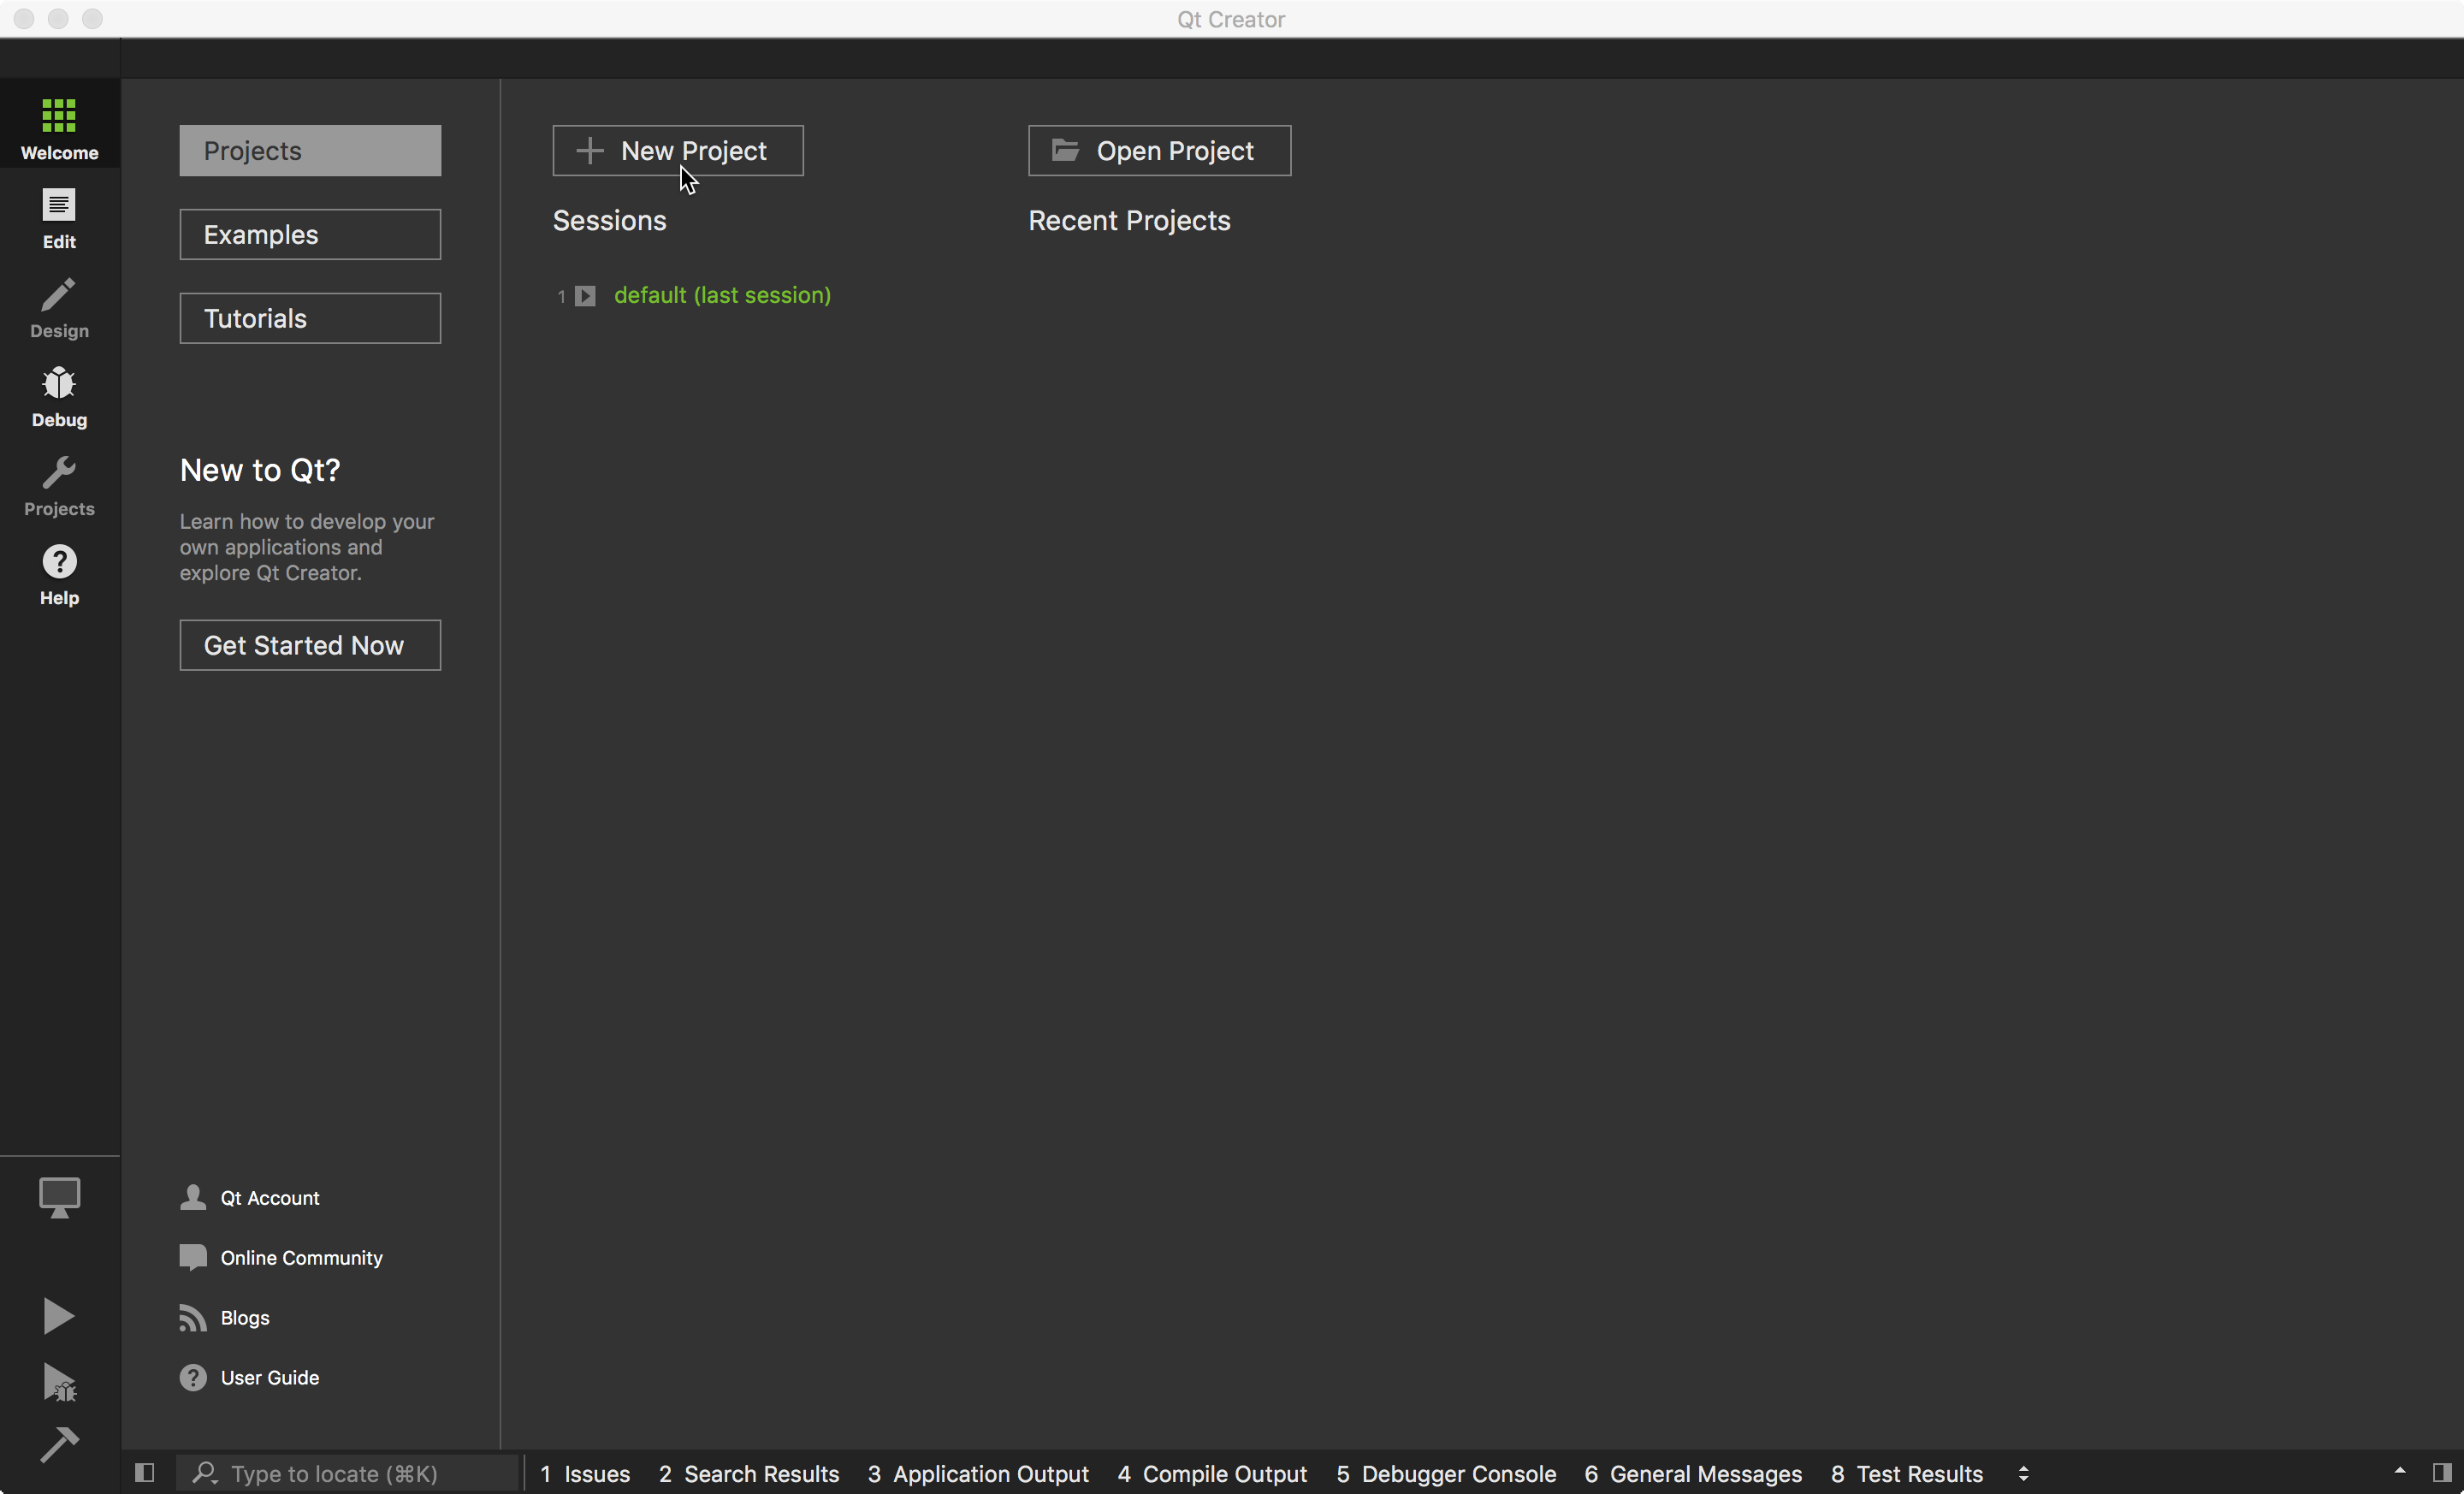
\includegraphics[width=\textwidth]{figures/new_project/select_new_project.png}
\end{figure}
You now choose a template. Select \textit{Non-Qt Project} in the sidebar to the left, then select \textit{Plain C++ Application} and click next.
\begin{figure}[H]
    \centering
    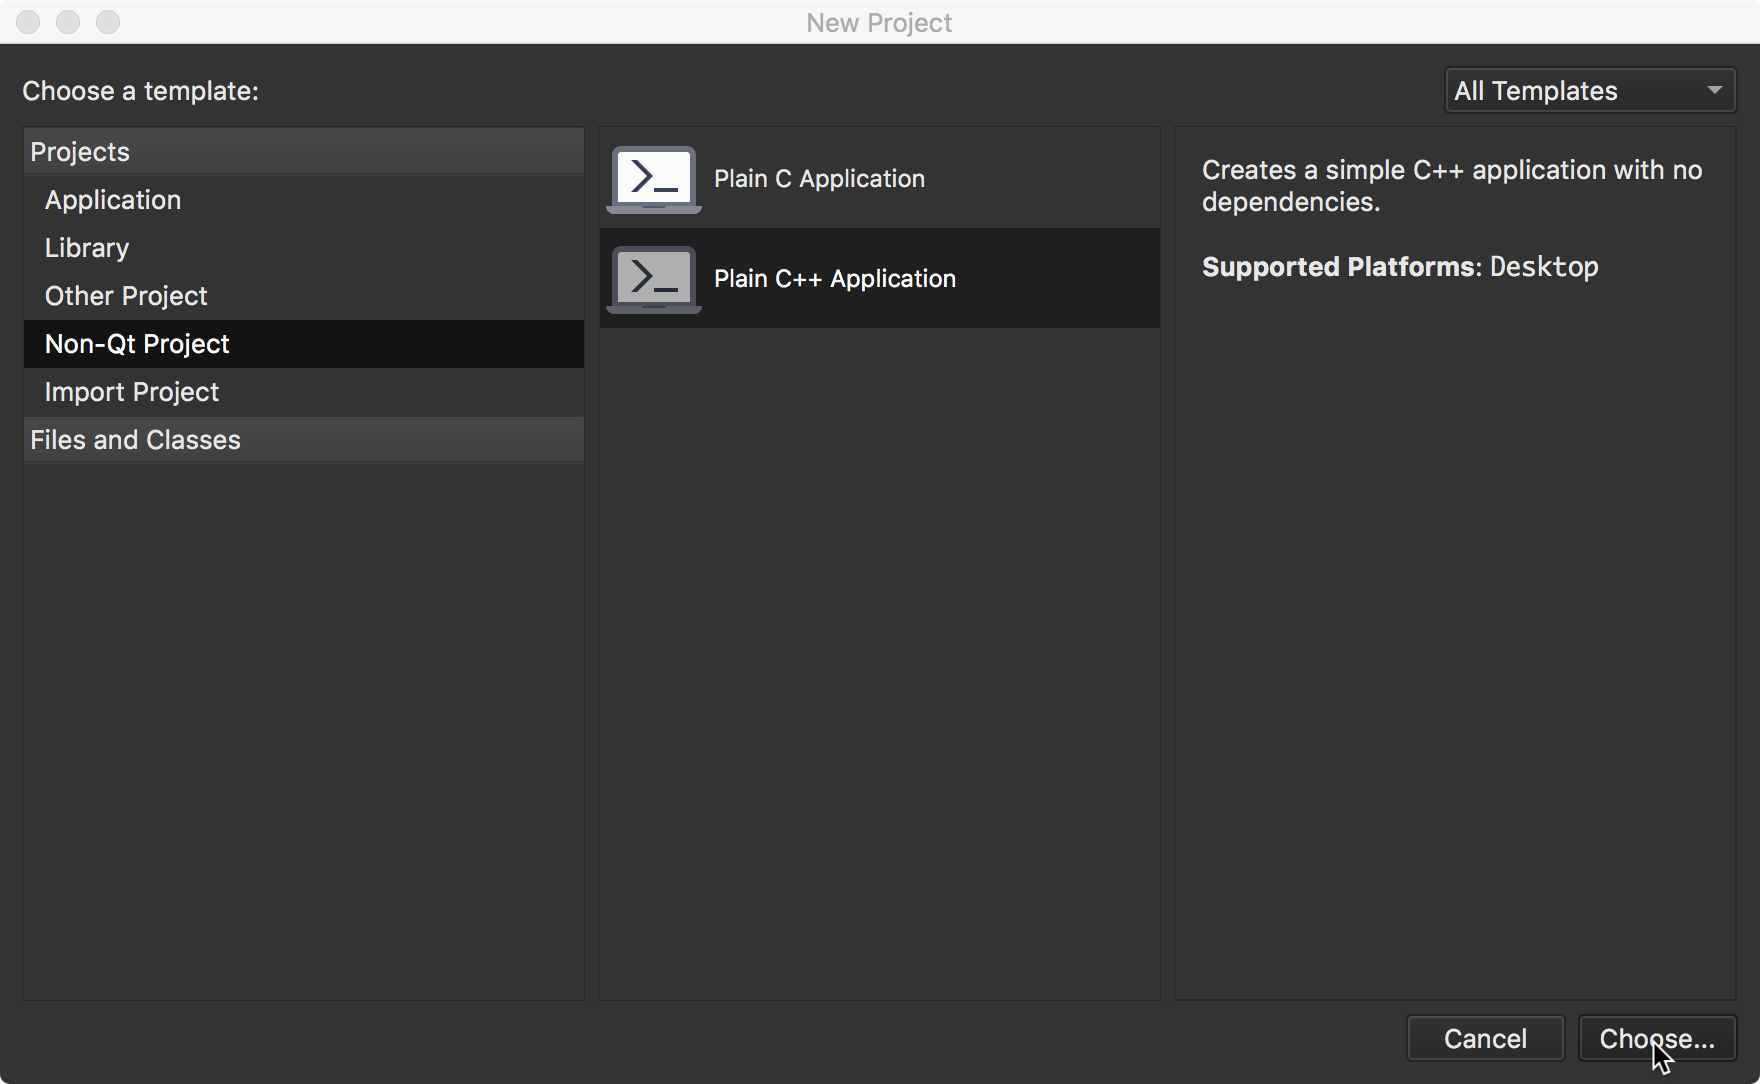
\includegraphics[width=\textwidth]{figures/new_project/non-qt-c++-app.png}
\end{figure}
Location. Then you give a name to your project and select its location.
\begin{figure}[H]
    \centering
    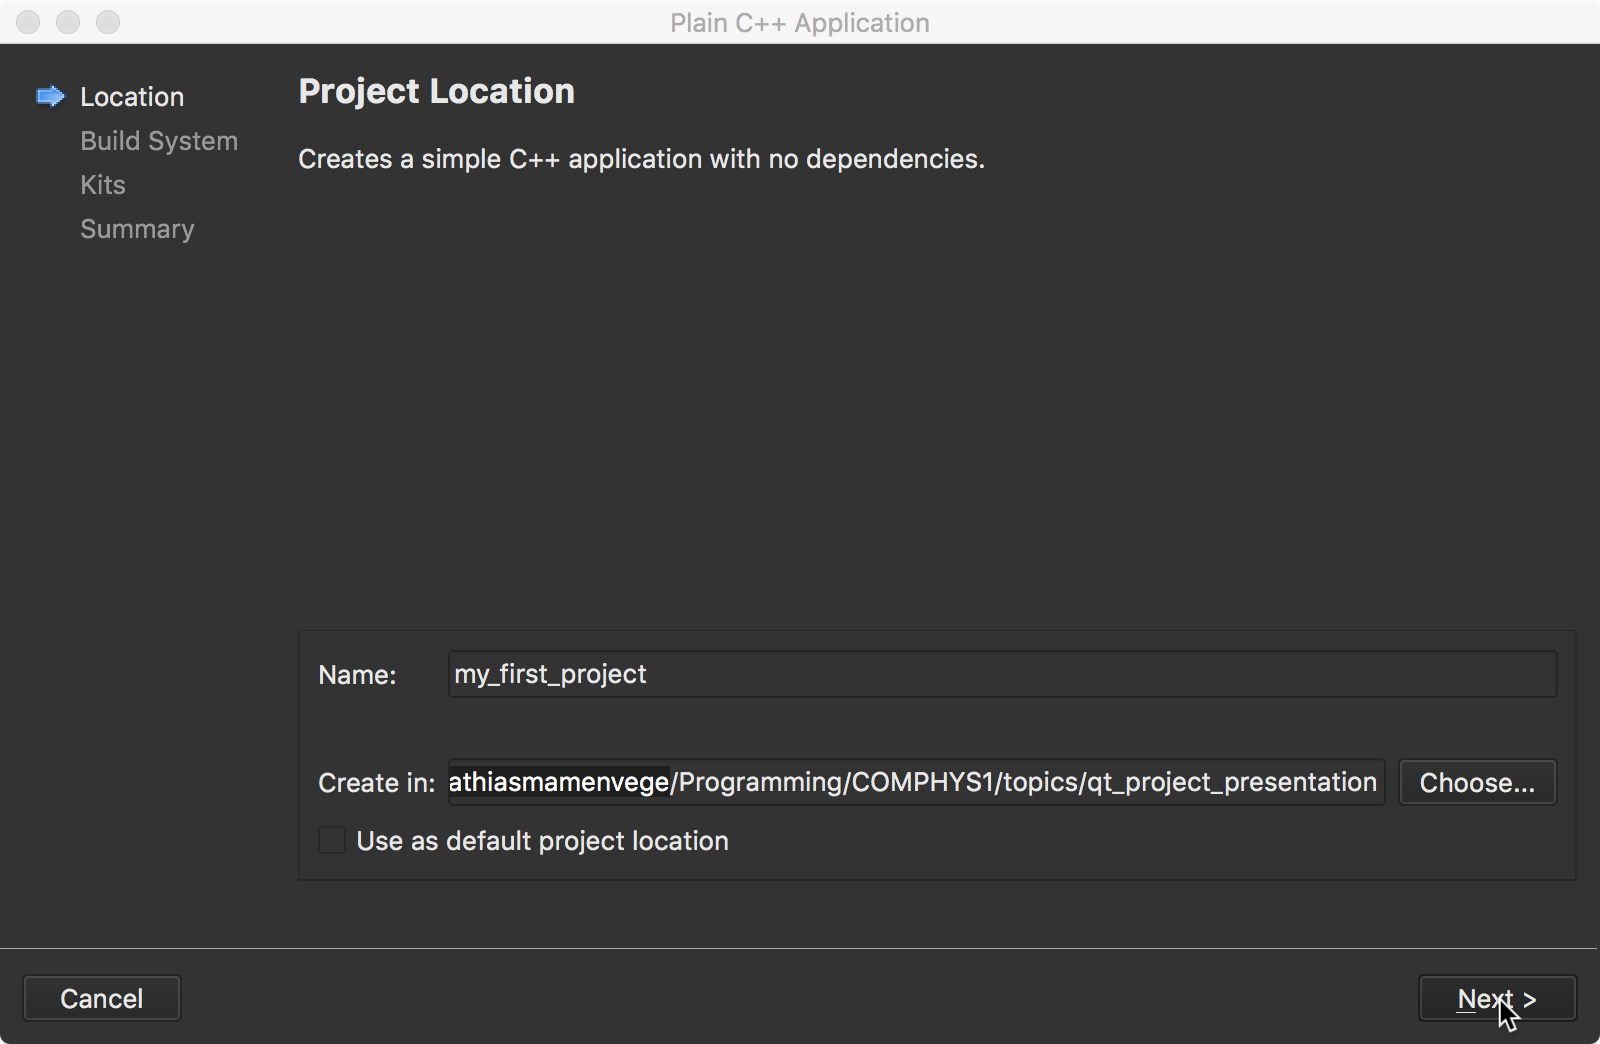
\includegraphics[width=\textwidth]{figures/new_project/select_folder_location.png}
\end{figure}
Build System. Default is \textit{qmake}, and is what we recommend.
\begin{figure}[H]
    \centering
    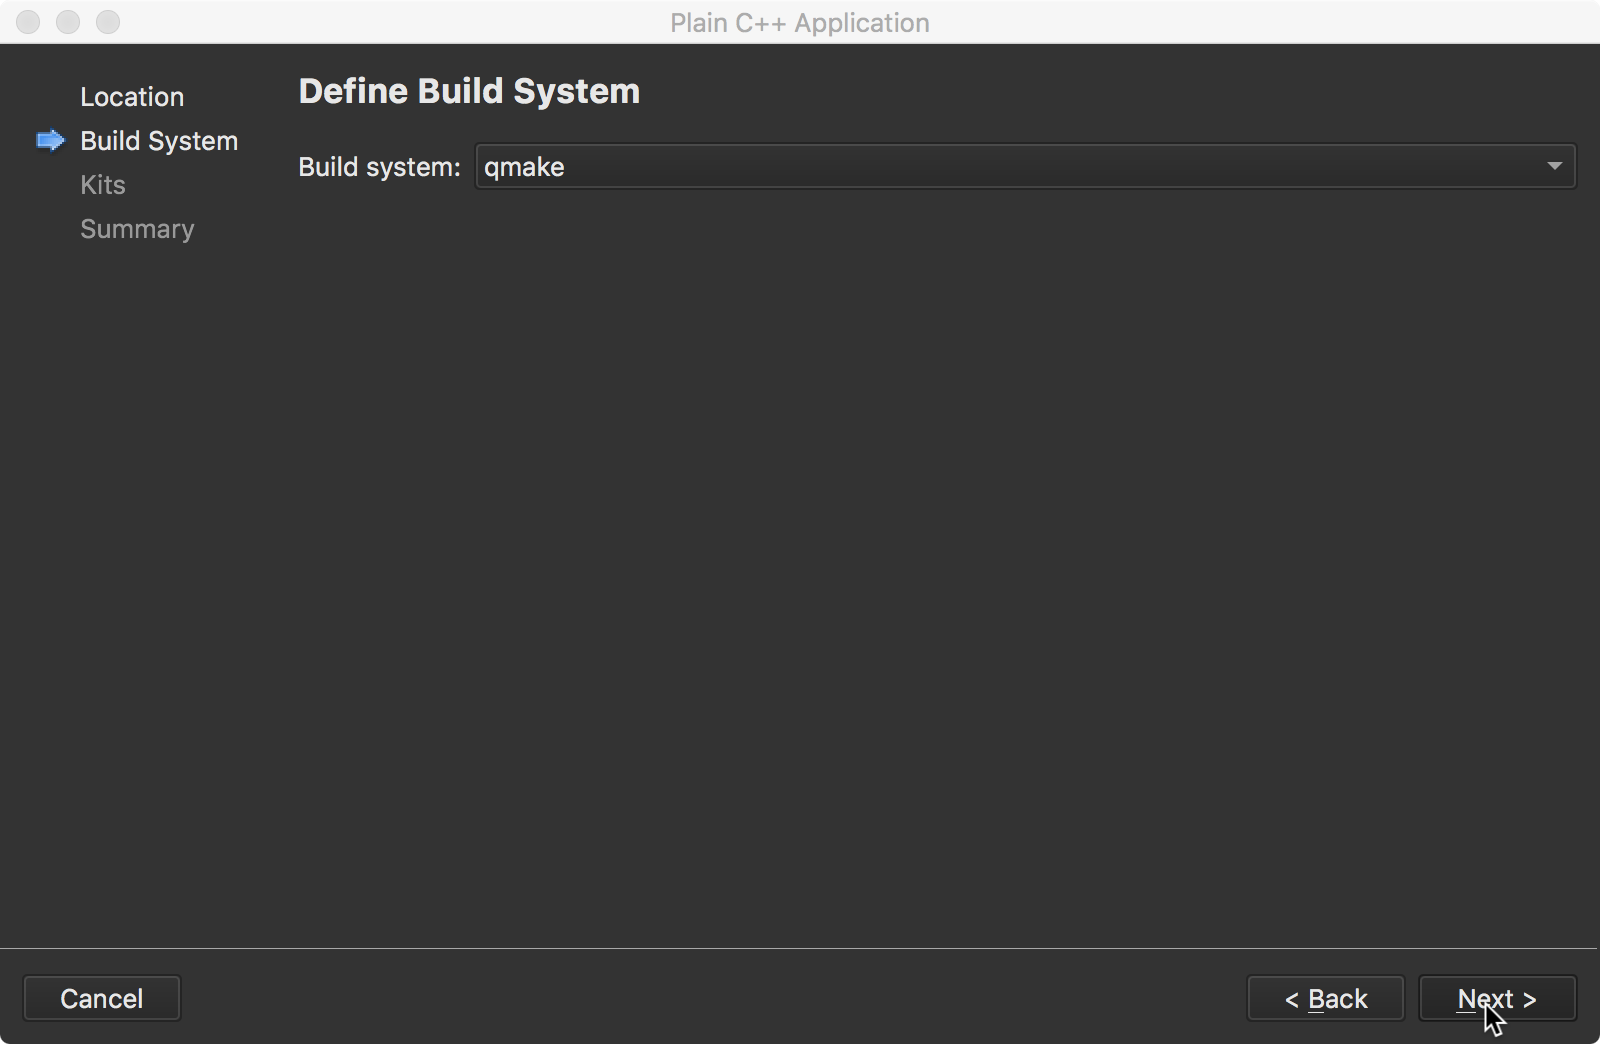
\includegraphics[width=\textwidth]{figures/new_project/default_build_system.png}
\end{figure}
Kit Selection. Select the newest kit available. May appear as \textit{Desktop}(on Ubuntu), \textit{Desktop Qt 5.11.1 clang 64bit}(on Mac) or similar. \textbf{Note:} if no kits are available, look back into the \textit{Installing Qt} section\ref{section:installing-qt}.
\begin{figure}[H]
    \centering
    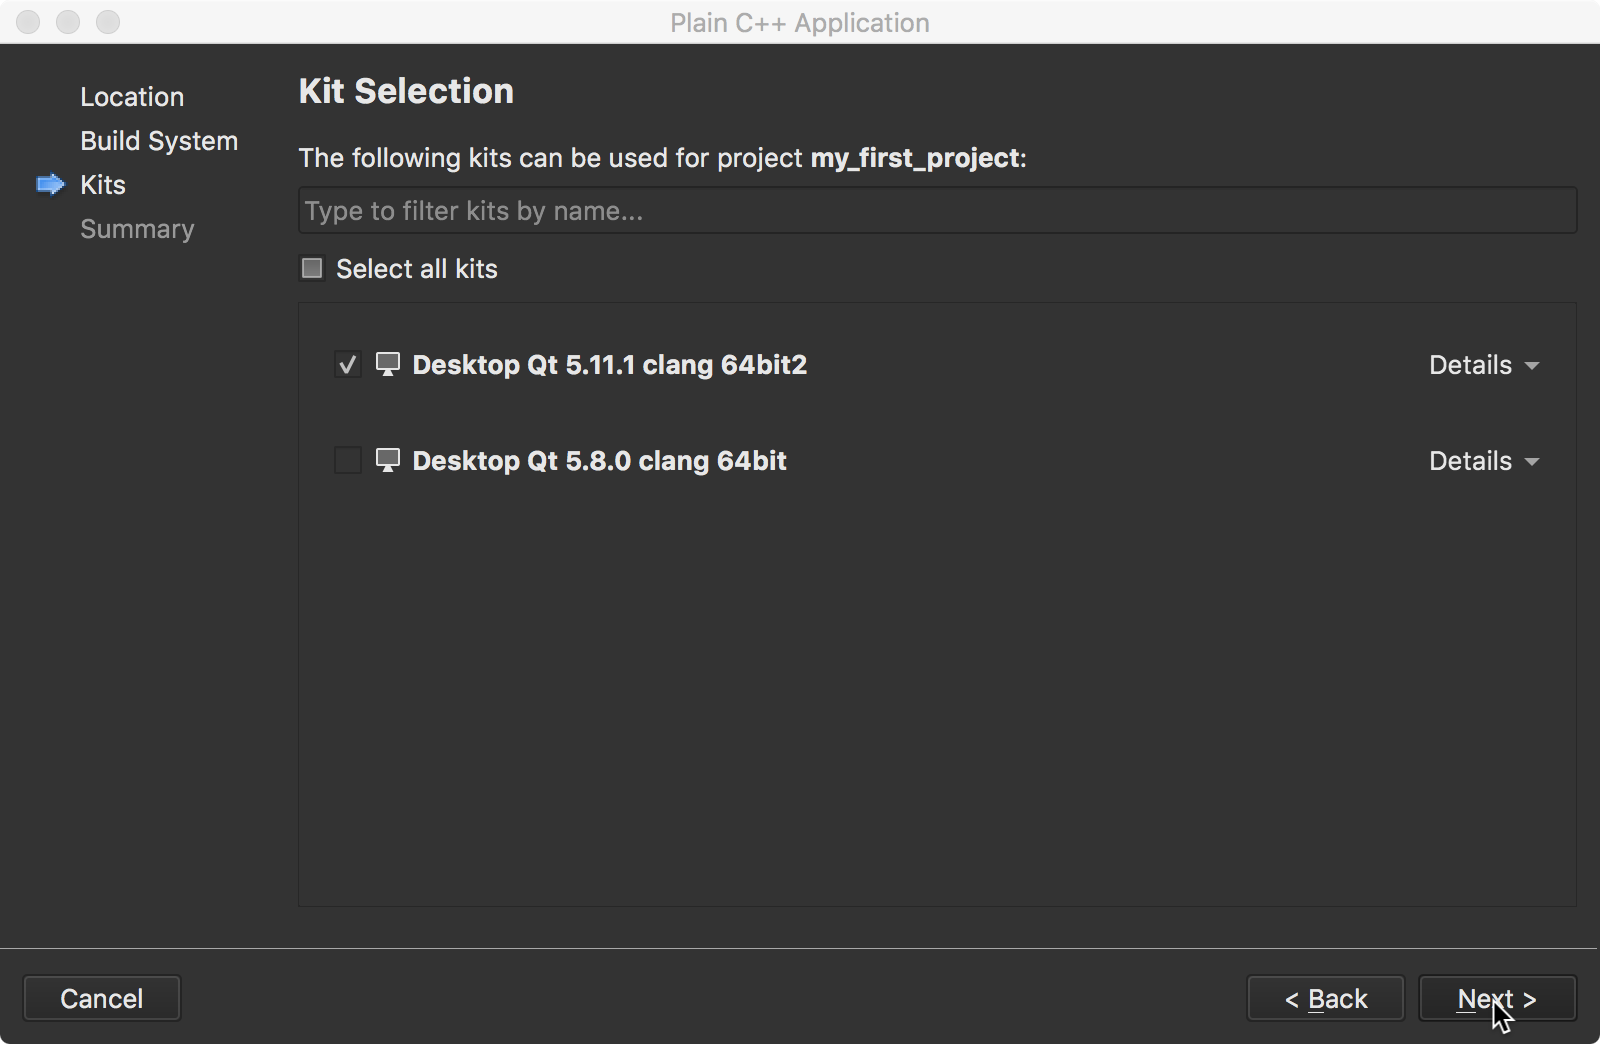
\includegraphics[width=\textwidth]{figures/new_project/select_kit.png}
\end{figure}
Summary. Everything should now be set up and ready to go, and you can begin programming.
\begin{figure}[H]
    \centering
    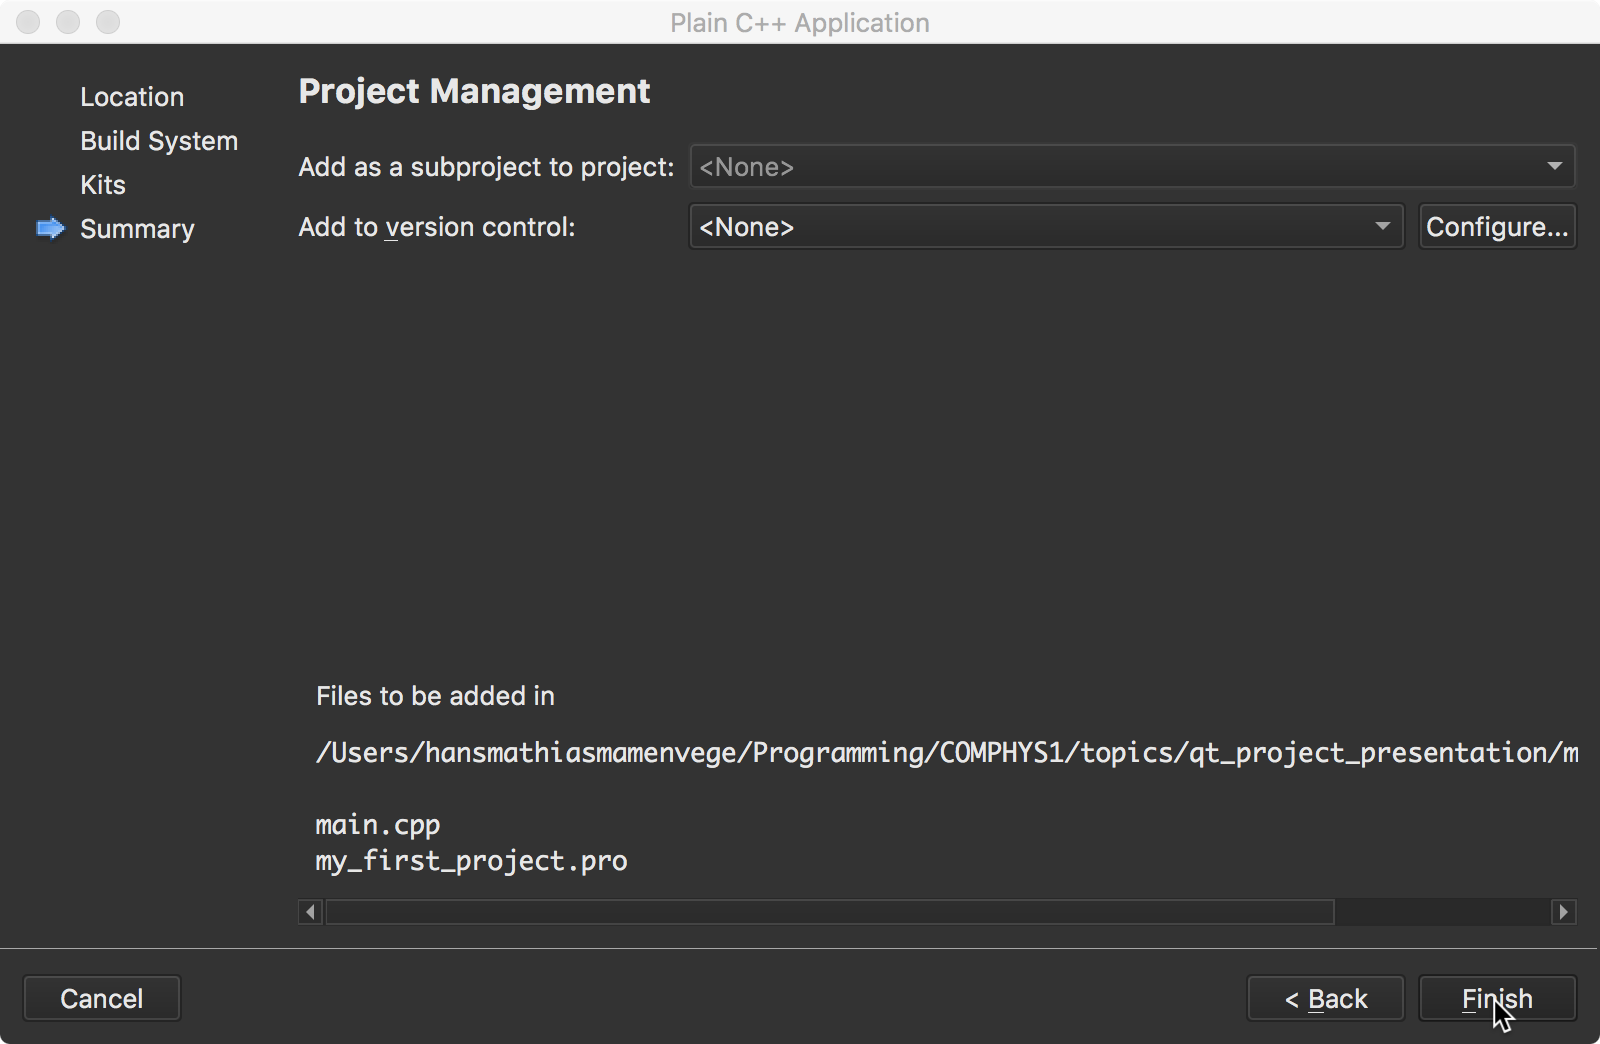
\includegraphics[width=\textwidth]{figures/new_project/summary.png}
\end{figure}
If you are missing a compiler, you might get a lot of errors under the \textit{Issues} panel. Go back to \textit{Installing Qt} section\ref{section:installing-qt} for how to install a compiler for your operating system.
\begin{figure}[H]
    \centering
    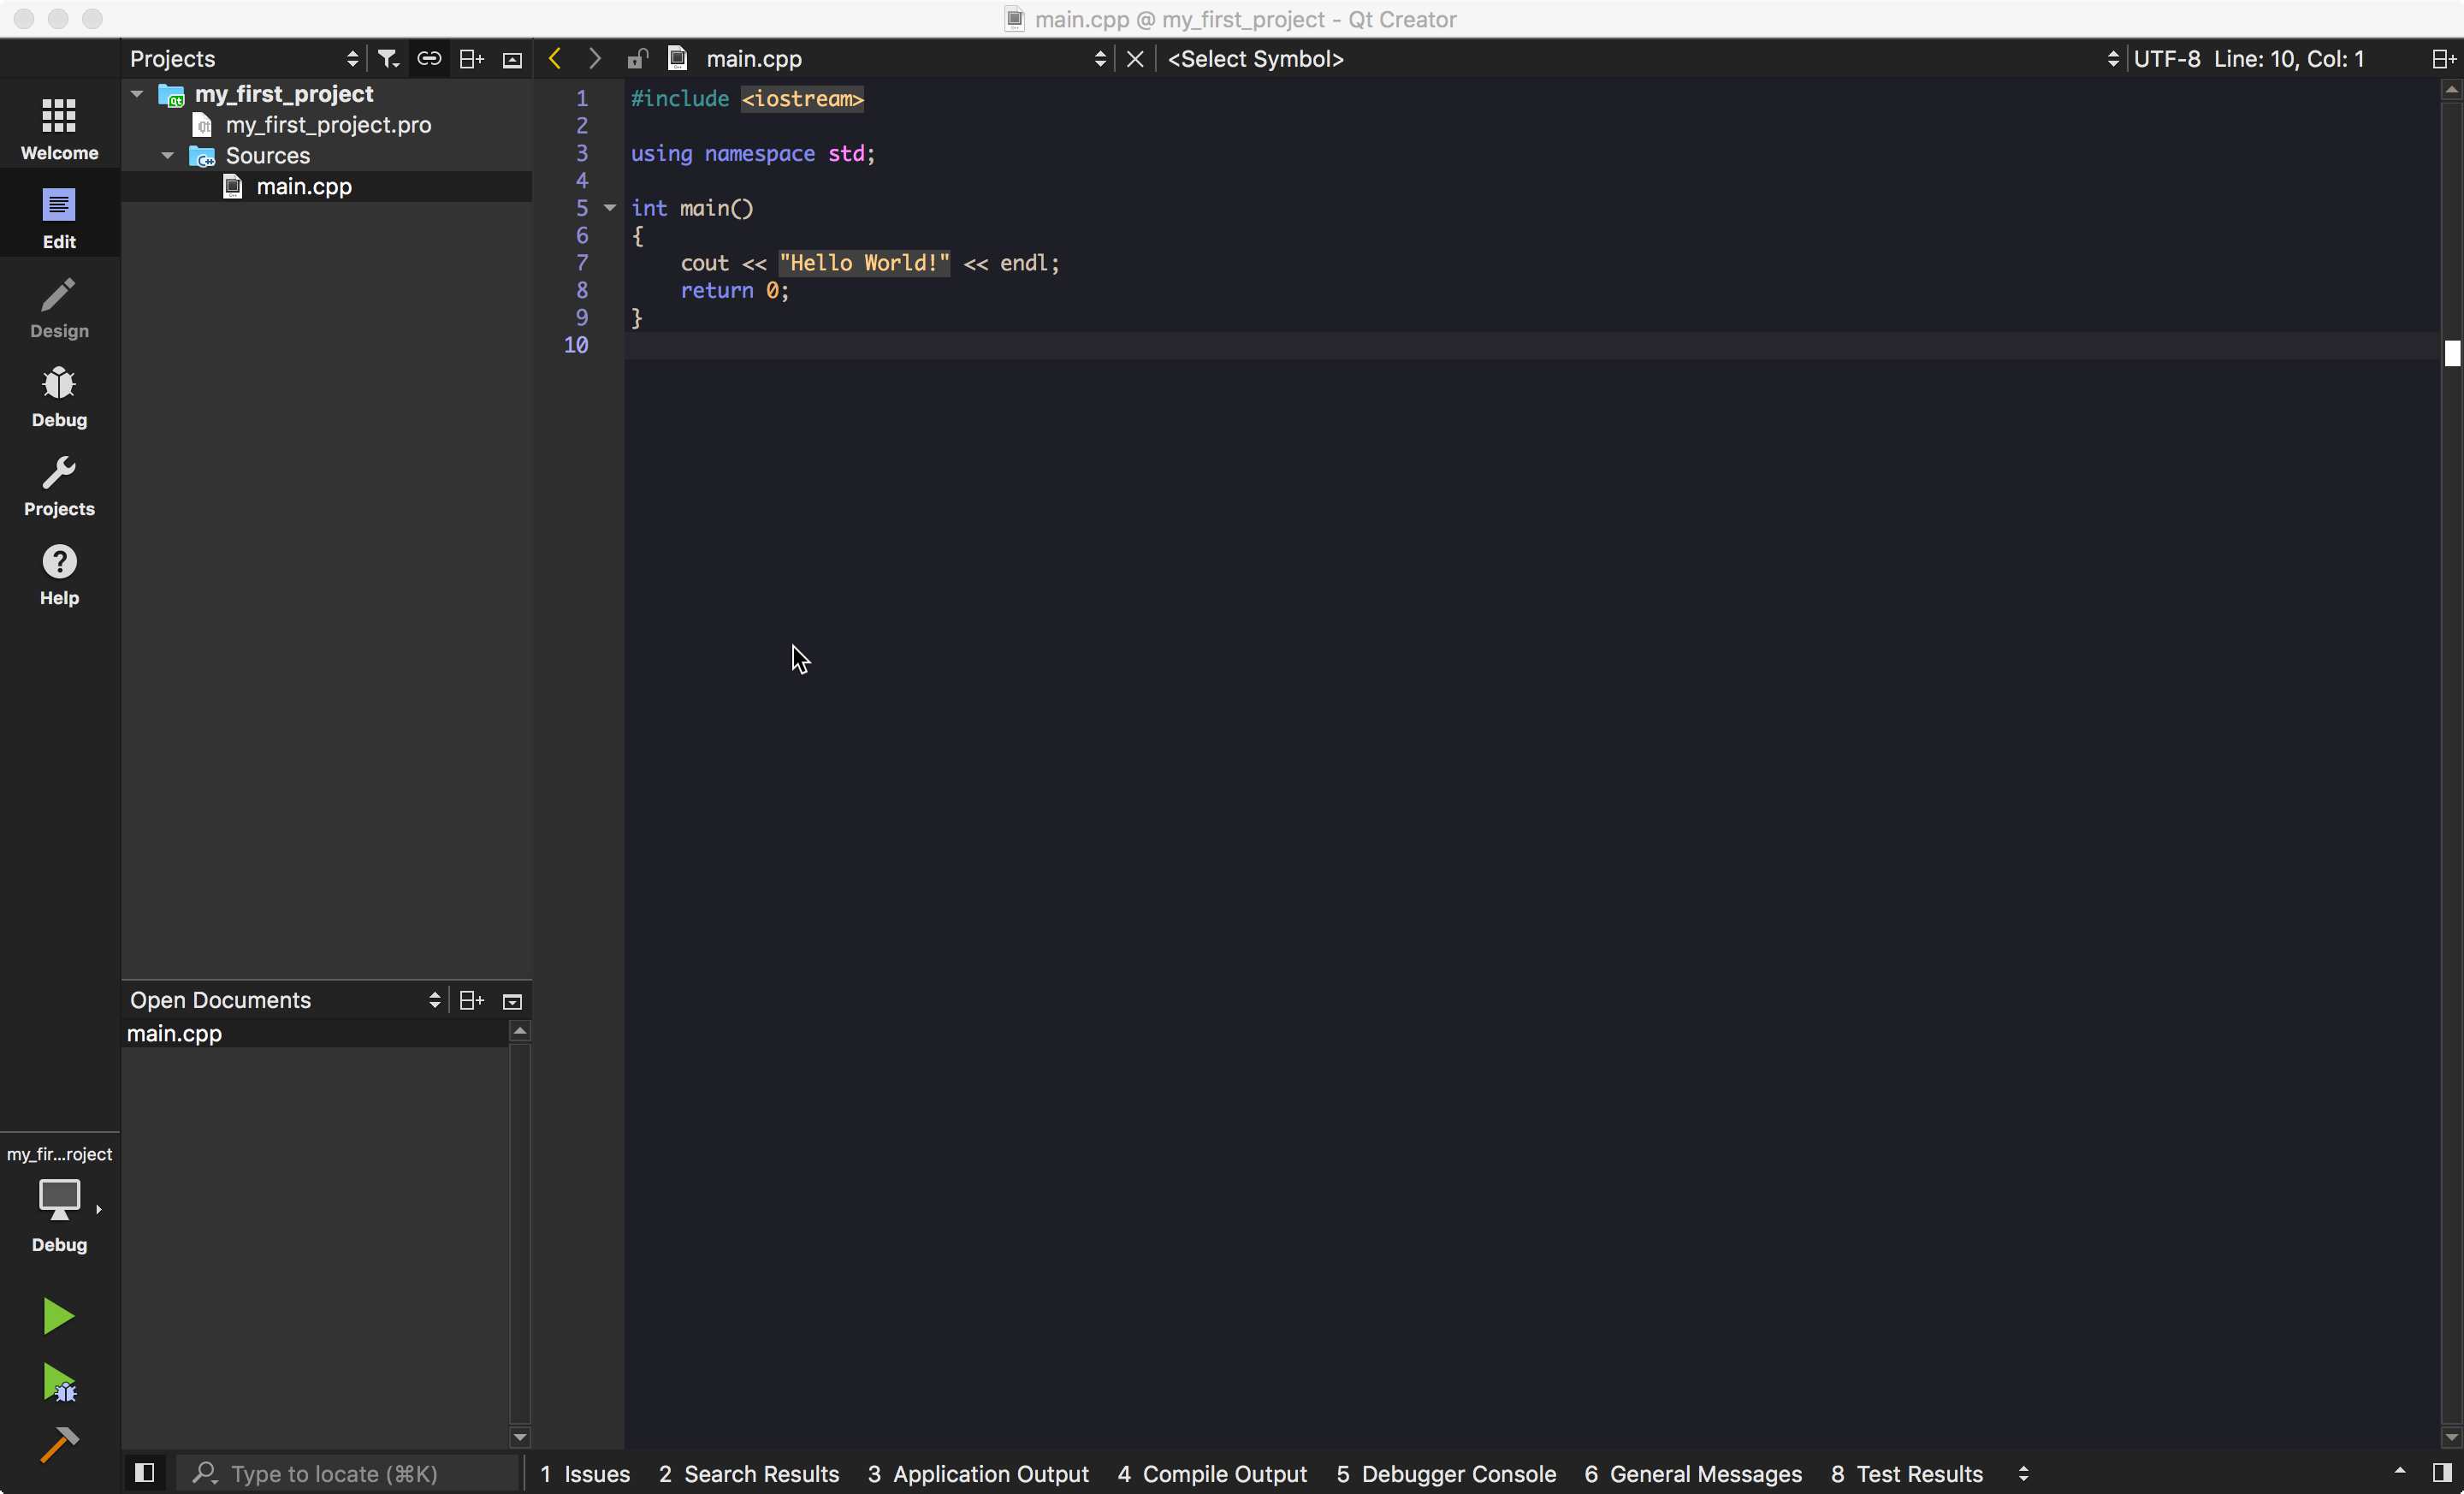
\includegraphics[width=\textwidth]{figures/new_project/edit_project_screen.png}
\end{figure}

\section{Project settings}
\subsection{Build settings}
A plethora of important settings can be accessed from the \textit{Build Settings} panel found in the side bar of Qt Creator.
\begin{figure}[H]
    \centering
    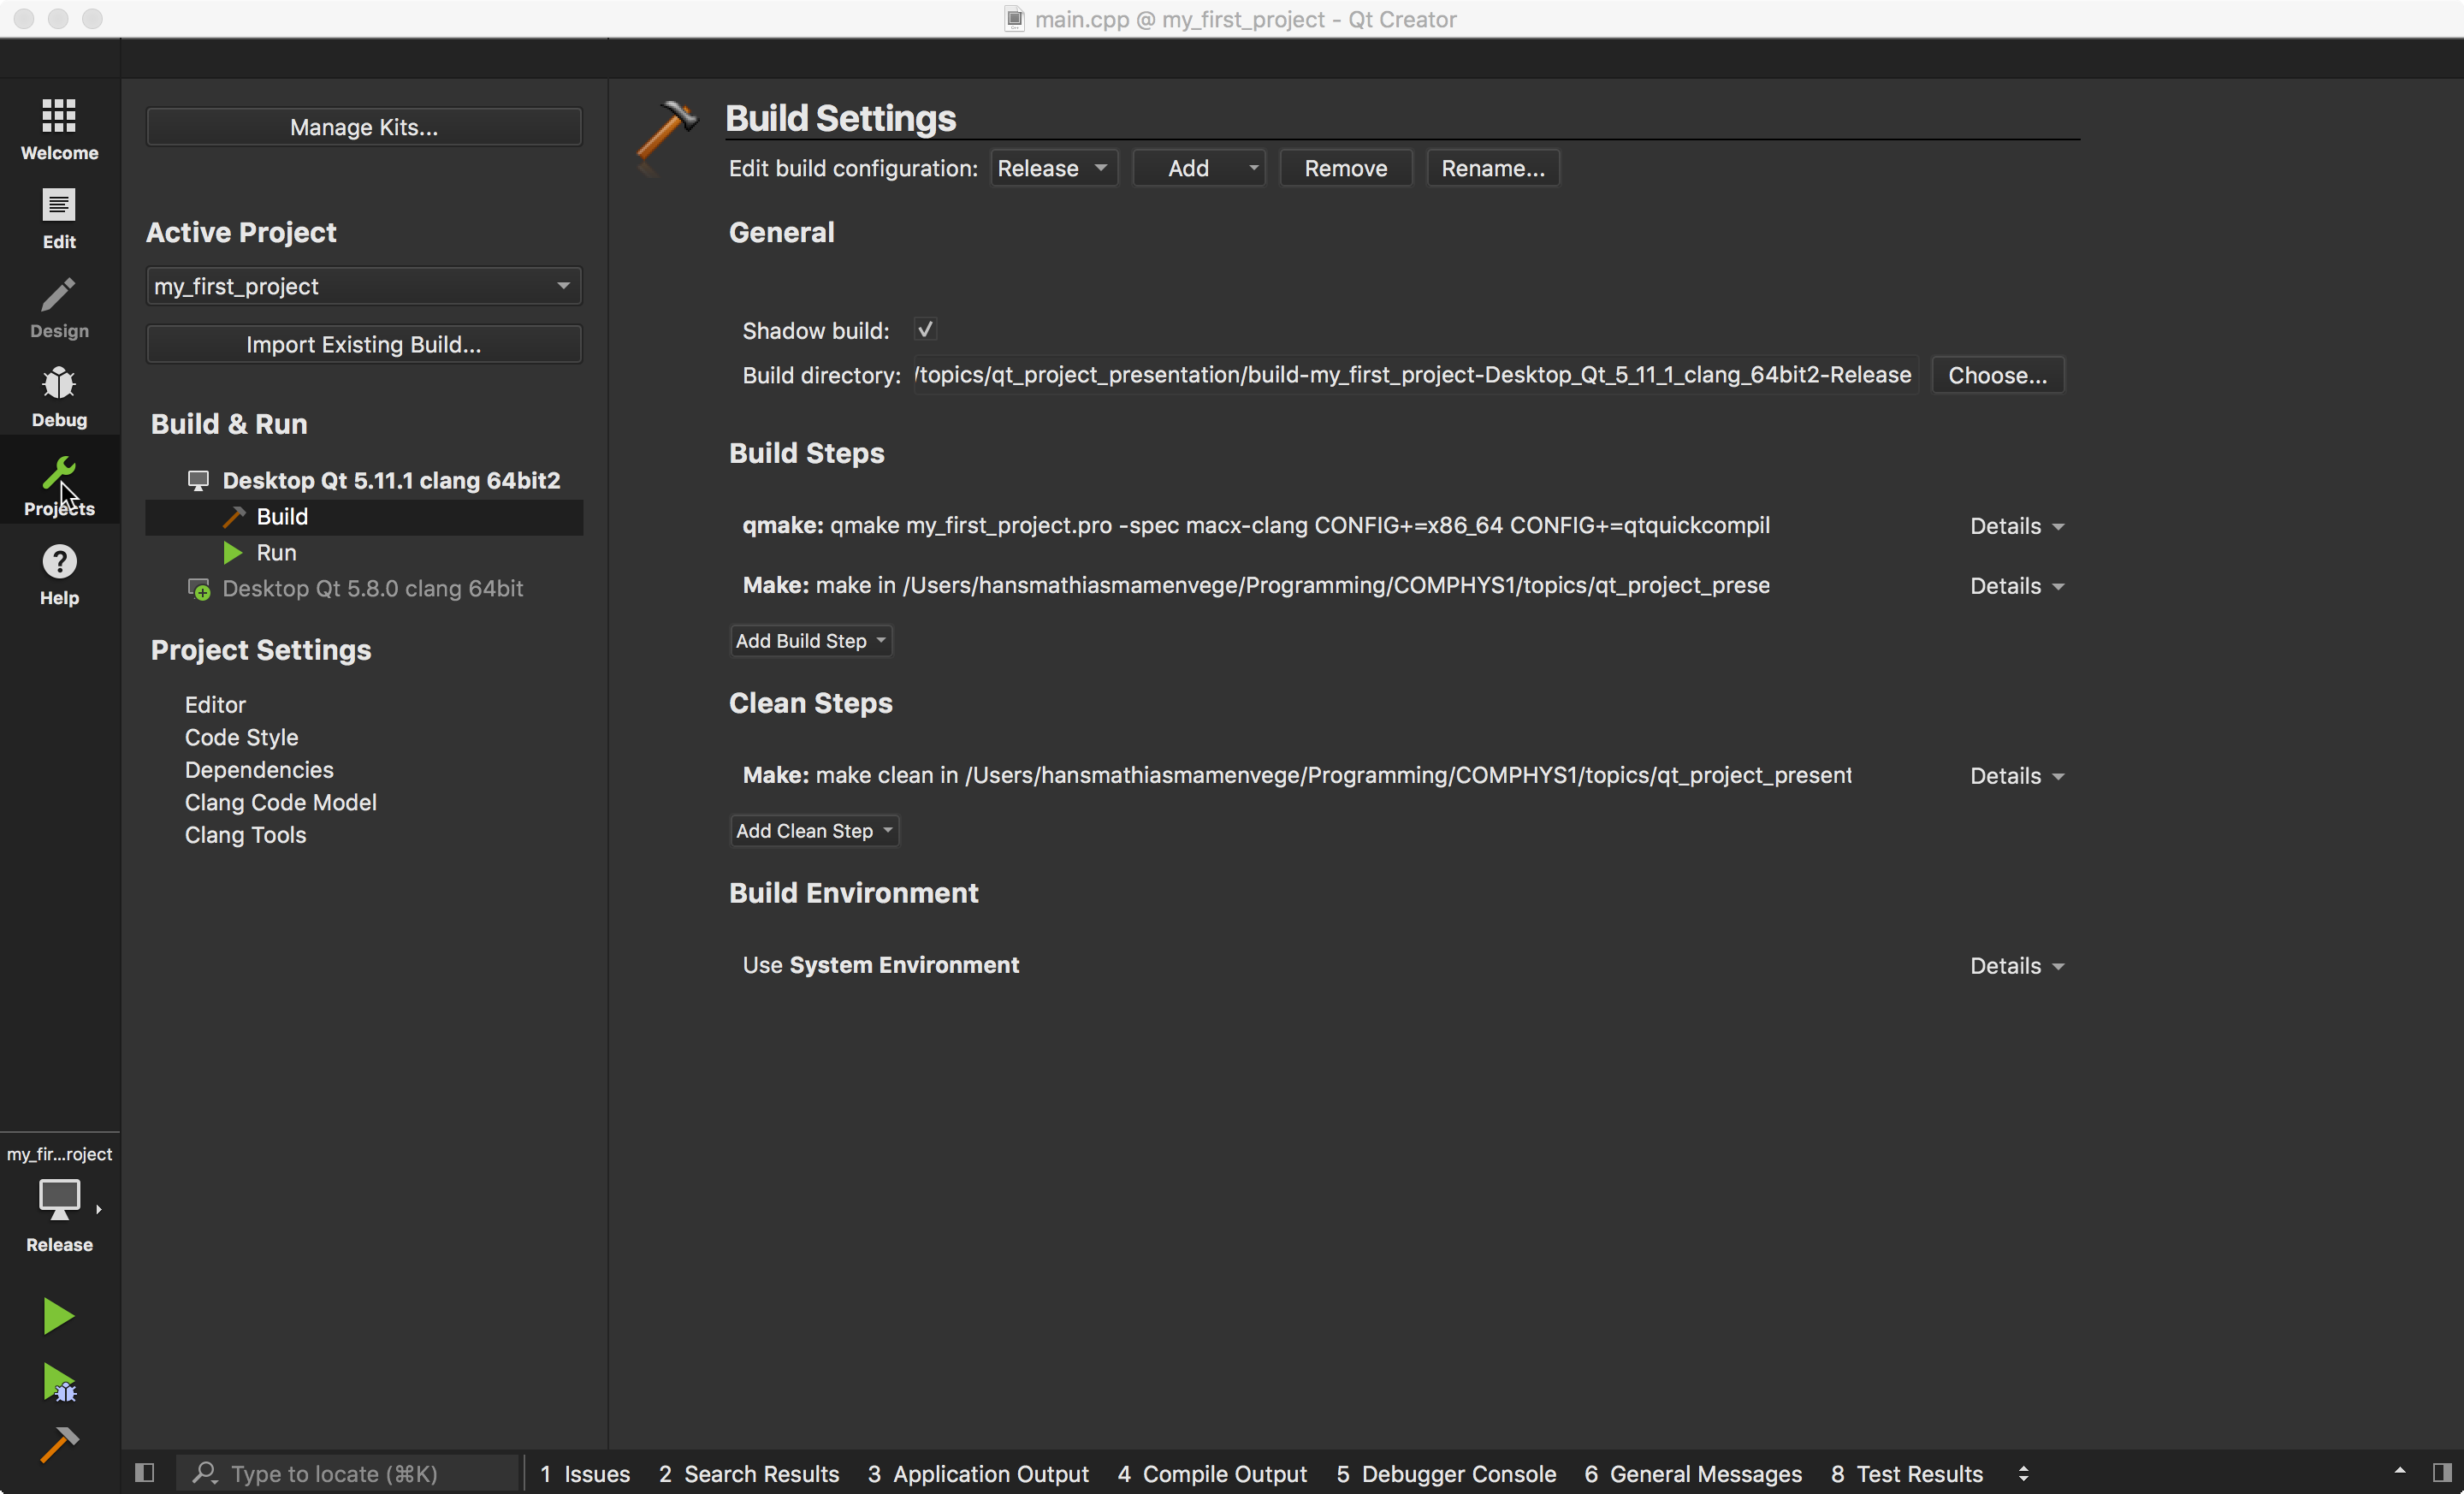
\includegraphics[width=\textwidth]{figures/changing_build_settings/build_settings_panel.png}
    \caption{Build settings panel.}
    \label{fig:build-settings}
\end{figure}
\subsection{Changing build folder}
By default, Qt Creator will create a build folder located one folder above the project folder.
\begin{lstlisting}
    \home\<user>\programming\my_project
    \home\<user>\programming\build-my_first_project-Desktop_Qt_5_11_1_clang_64bit2-Release
    \home\<user>\programming\build-my_first_project-Desktop_Qt_5_11_1_clang_64bit2-Profiling
    \home\<user>\programming\build-my_first_project-Desktop_Qt_5_11_1_clang_64bit2-Debug
\end{lstlisting}
It will typically make on folder for each of the \texttt{Release}, \texttt{Debug} and \texttt{Profiling} builds. If you want to change this go to the settings folder as listed in the figure above \ref{fig:build-settings}. This can be changed under the \textit{General} section, by selecting a \textit{build directory} depending on what build you are currently set to,
\begin{figure}[H]
    \centering
    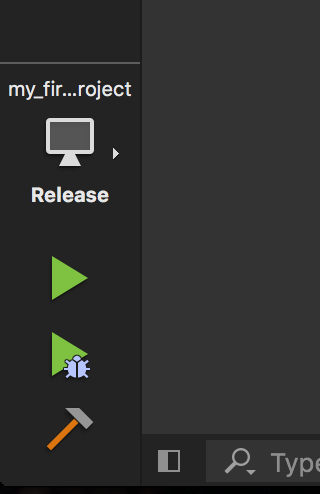
\includegraphics[scale=0.4]{figures/changing_build_settings/build_select.png}
    \caption{Build selecting found in the lower left corner.}
    \label{fig:build-selection}
\end{figure}

\subsection{Run settings}
If we now click the \textit{Run Settings} as seen on the \textit{Build Settings} panel, we get the following screen up,
\begin{figure}[H]
    \centering
    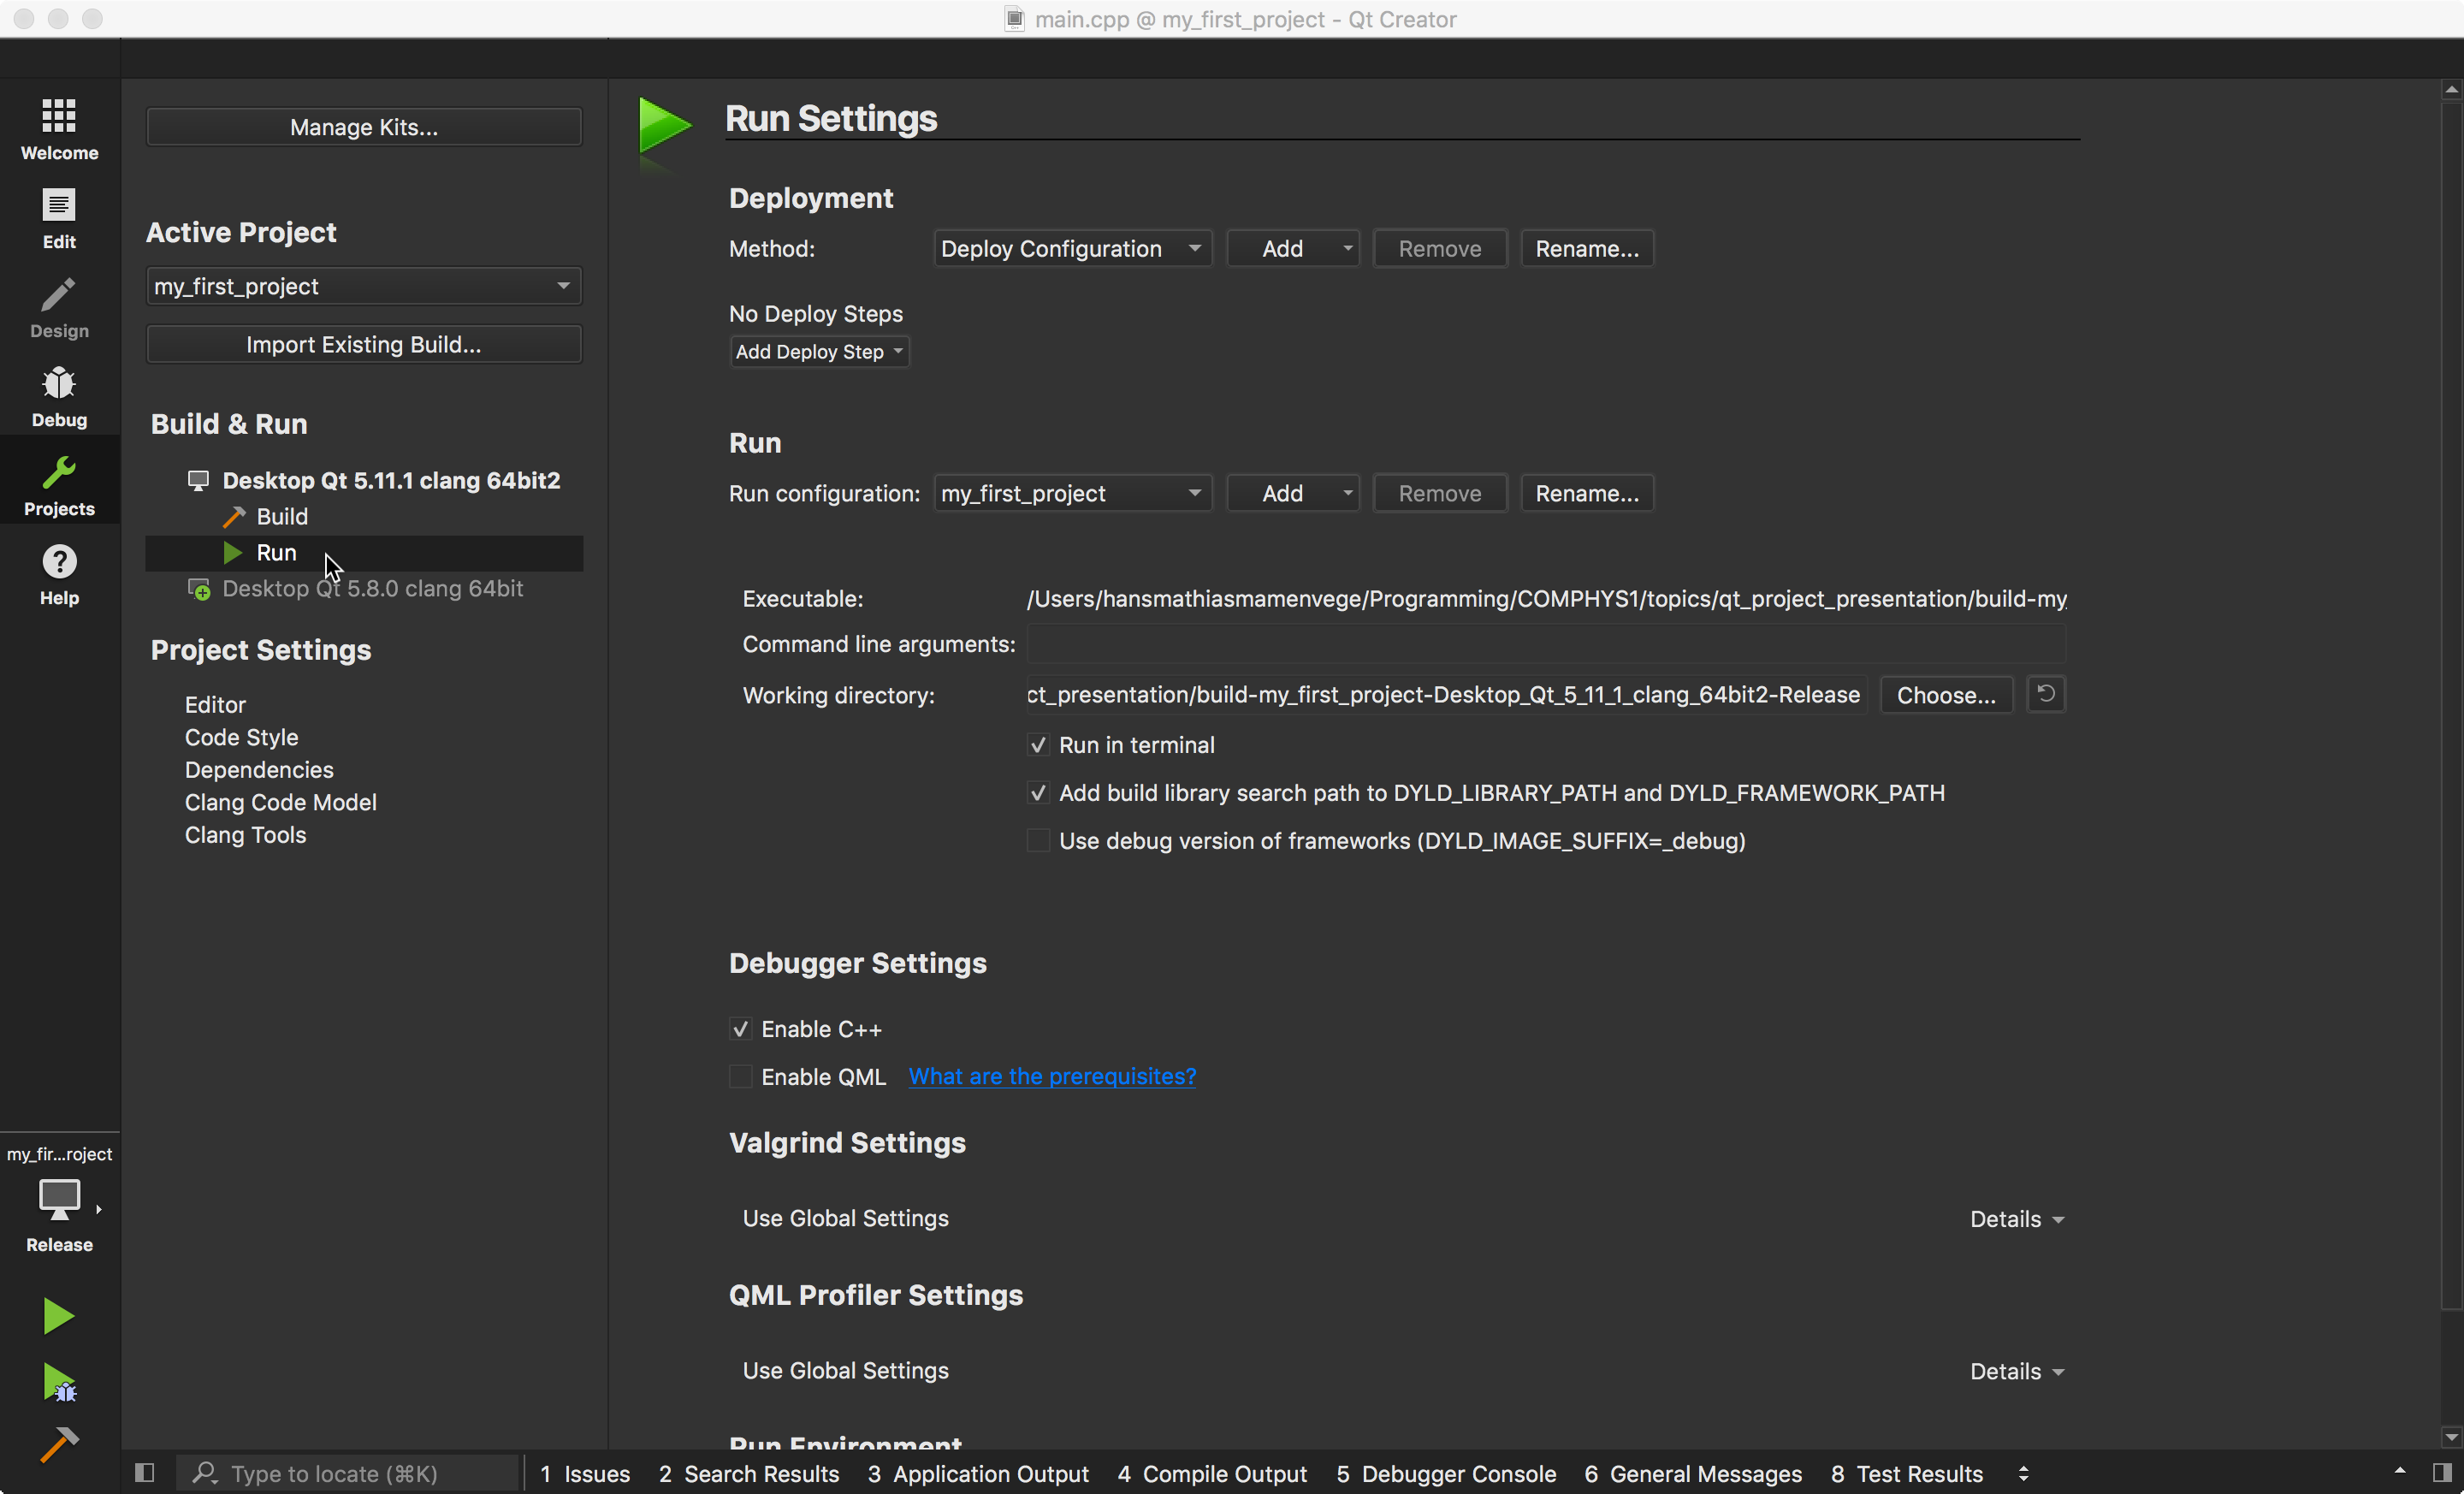
\includegraphics[width=\textwidth]{figures/changing_build_settings/run_settings_panel.png}
    \caption{Run settings panel found at under the build settings panel\ref{fig:build-settings}.}
    \label{fig:run-settings}
\end{figure}
\subsection{Command line arguments}
If you want to add command line arguments to your program, there are two ways of doing it. One is to run the program from the terminal in a regular fashion,
\begin{lstlisting}
    $ ./my_first_project arg1 arg2 arg3 
\end{lstlisting}
Or, you can add the arguments under \textit{Run} section in the \textit{Command line arguments},
\begin{figure}[H]
    \centering
    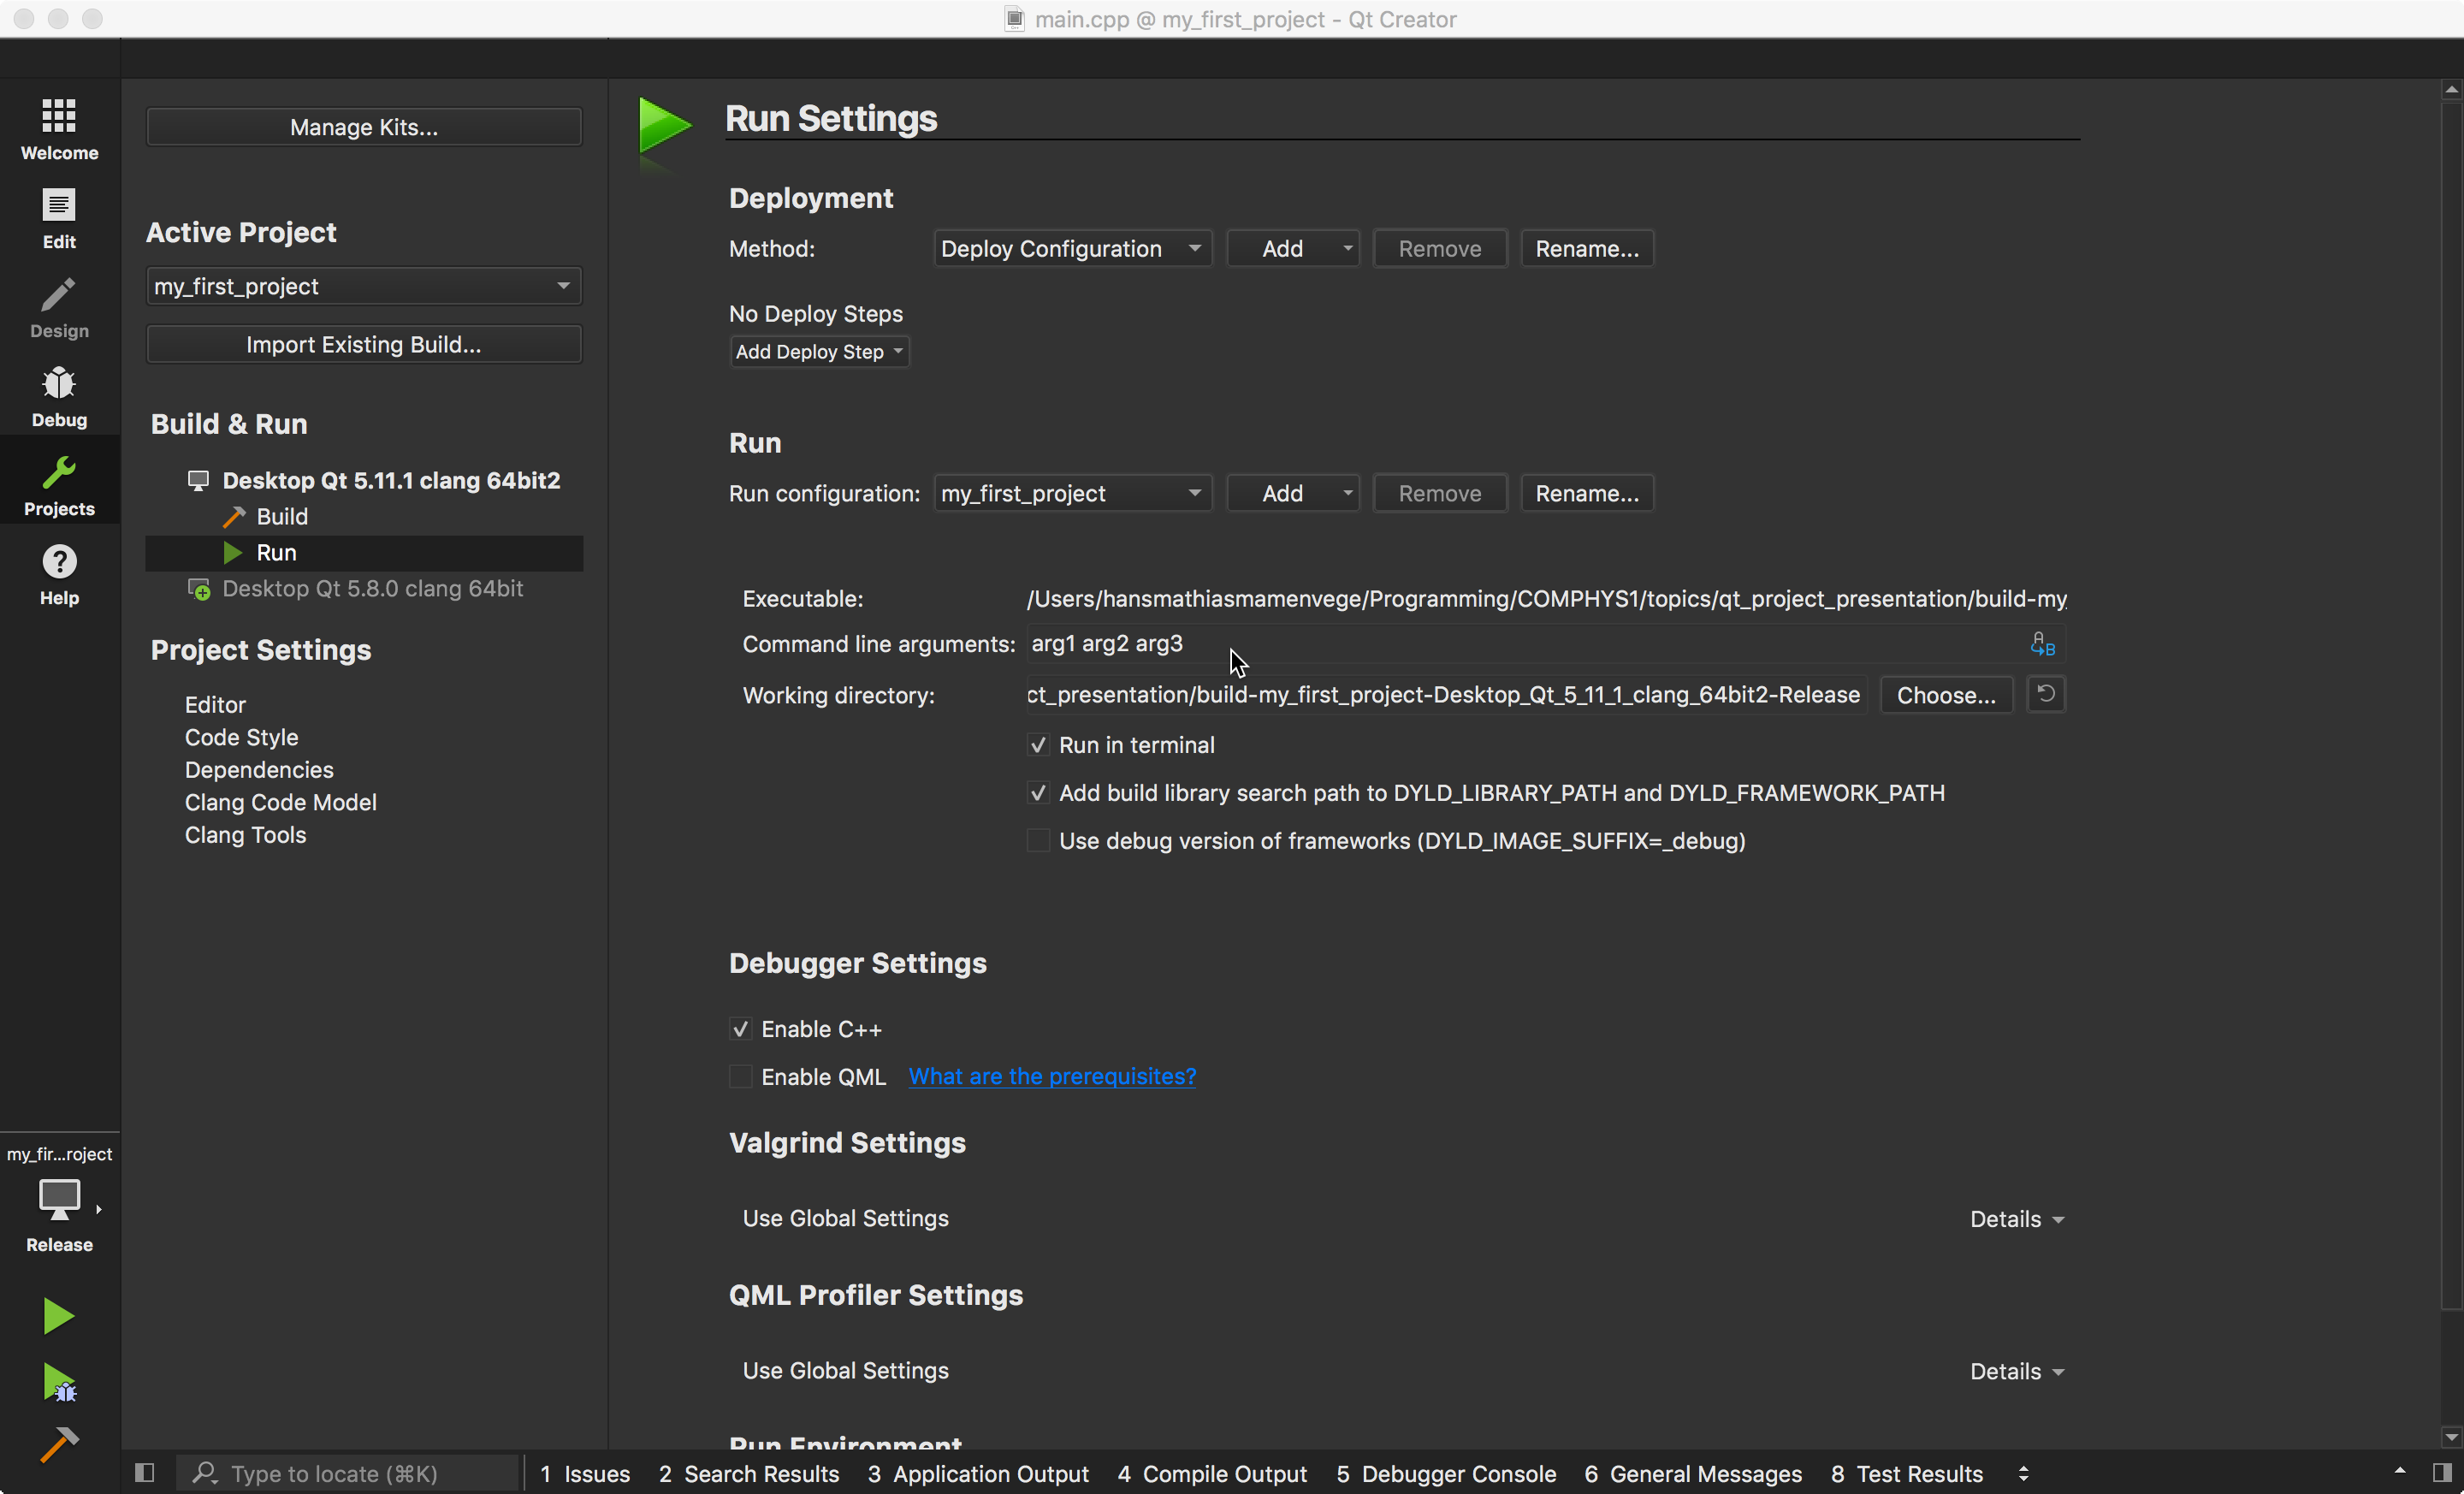
\includegraphics[width=\textwidth]{figures/changing_build_settings/arguments.png}
\end{figure}
You can also turn of the \textit{Run in terminal} mode by unchecking the box slightly below the \textit{Command line arguments} input.
\begin{lstlisting}
    $ ./my_first_project arg1 arg2 arg3 
\end{lstlisting}

\section{Expanding your project}
\subsection{The \texorpdfstring{\texttt{.pro}}{.pro}-file}
The \texttt{.pro} contains the settings for QMake, which is the compiling tool used by Qt(instead something like cmake). Your \texttt{.pro} file will look like this at the beginning of your project,
\lstinputlisting[style=custom-pro-file]{example_project_files/my_first_project.pro}
From the \texttt{.pro} file you can specify what \CC version you are going to use(\CC11 should be the default), what optimizations to utilize and what external libraries we are to use.

\subsection{Adding files and classes}
When adding new files to your project, either
\begin{itemize}
    \item press \texttt{CMD+N}.
    \item click \textit{New File} under \textit{File}
    \item right click at the folder you wish to create a new file in the \textit{Projects} tab and select \textit{Add New...}.
\end{itemize}
If you do either of the of the first two you should get up a panel similar to the one you got when starting a new folder. Instead of looking under the \textit{Projects} templates, go beneath that to \textit{Files and Classes} and select \textit{C++}. Then select the type of file you are going to choose,
\begin{figure}[H]
    \centering
    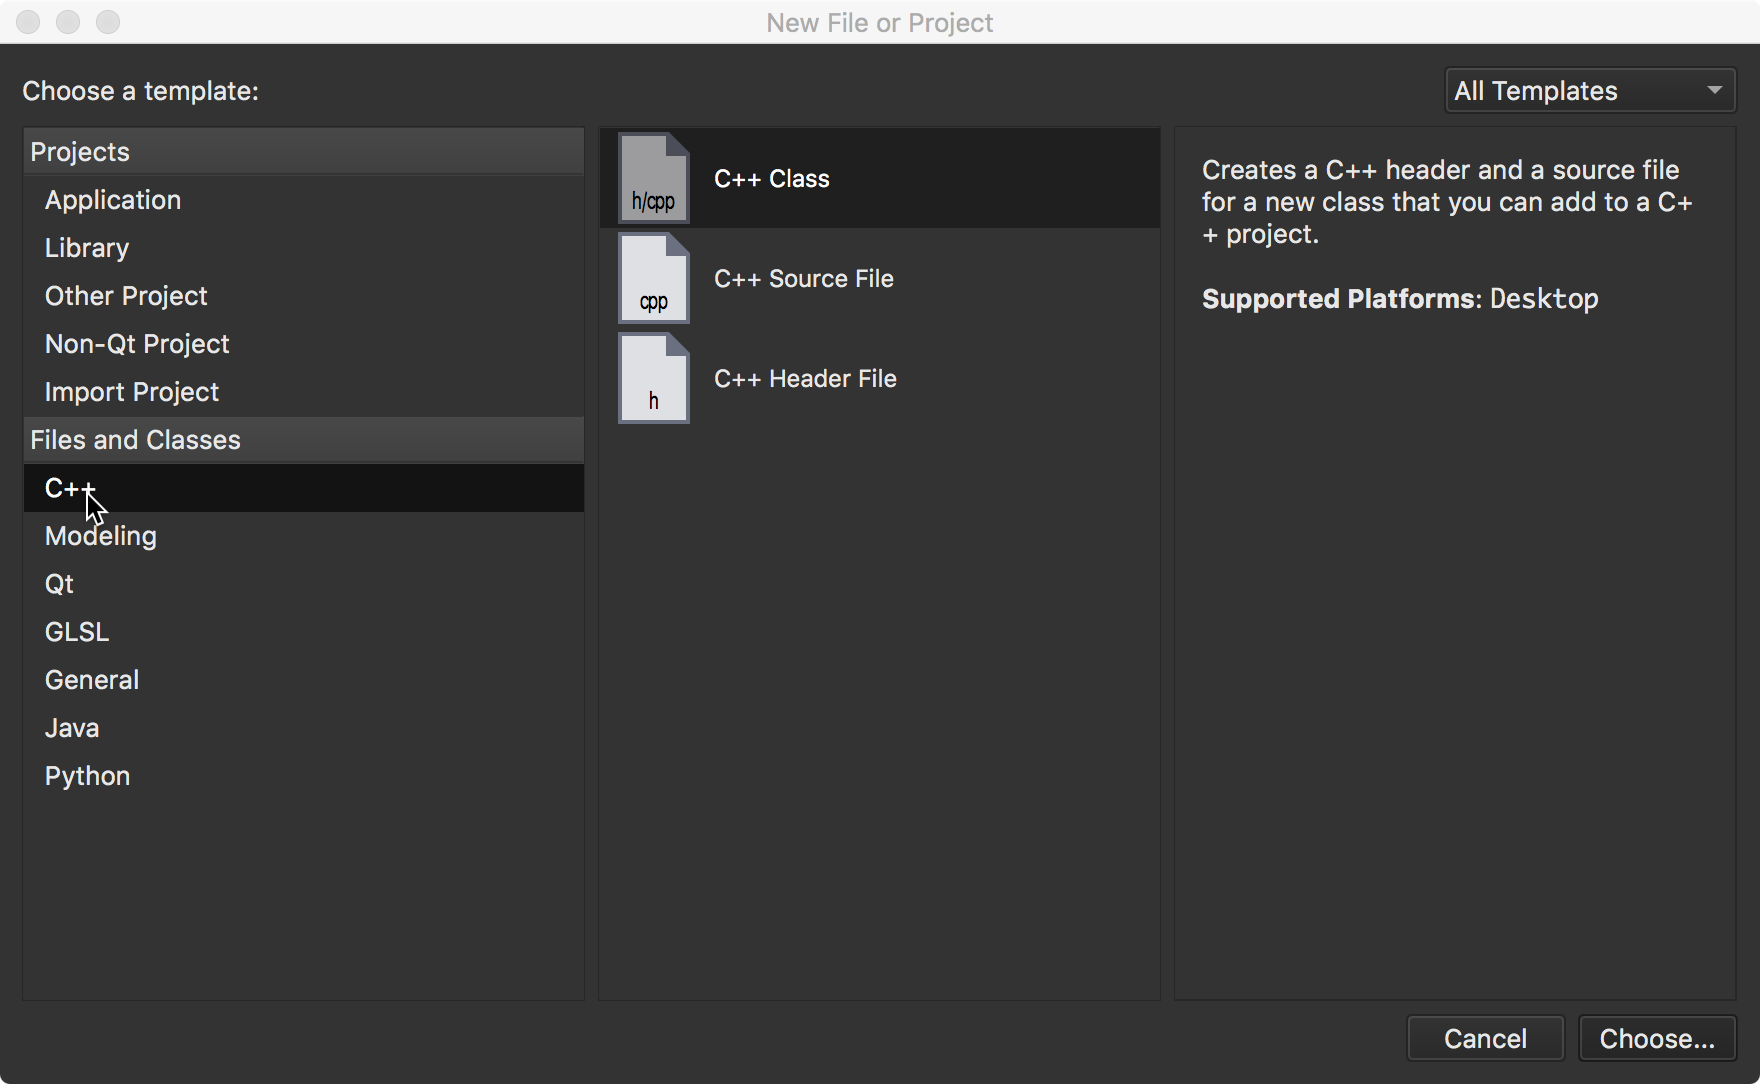
\includegraphics[width=\textwidth]{figures/new_files/select_file.png}
\end{figure}
\subsubsection{New header files}
If you are going to create a header, select that and give it a name and location in the next panel. The summary screen will then look something like this,
\begin{figure}[H]
    \centering
    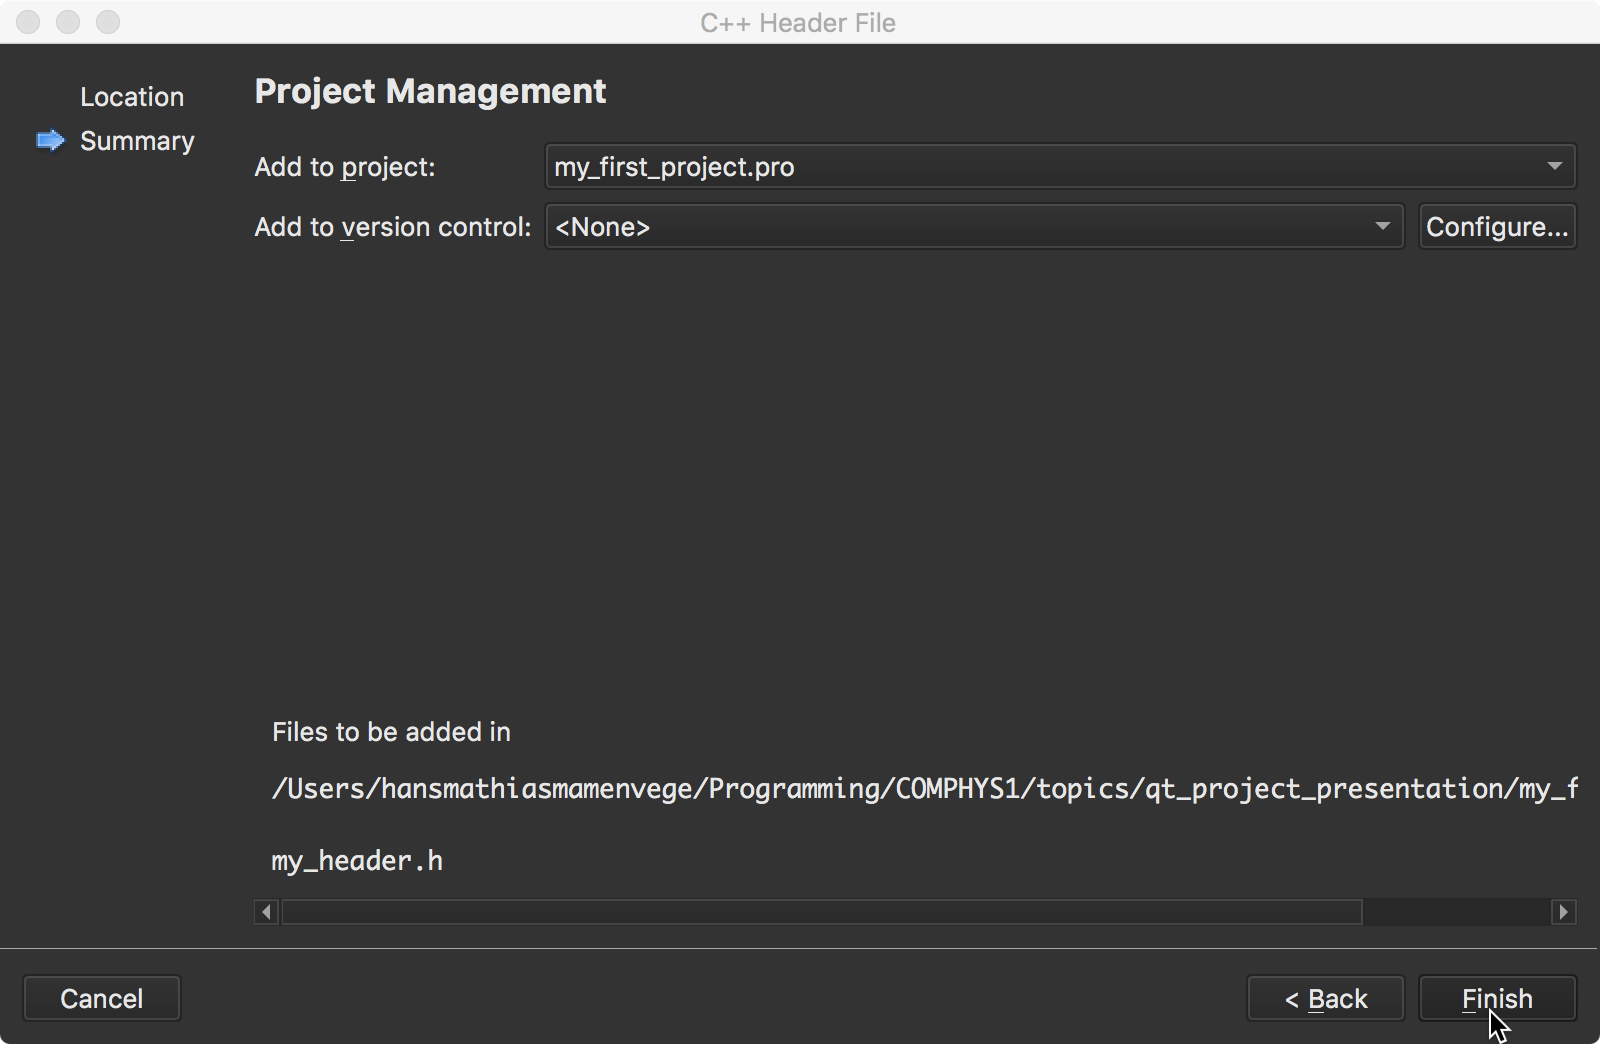
\includegraphics[width=\textwidth]{figures/new_files/first_header.png}
\end{figure}
\subsubsection{New Classes}
If you are setting up a class, select that and give it a name.
\begin{figure}[H]
    \centering
    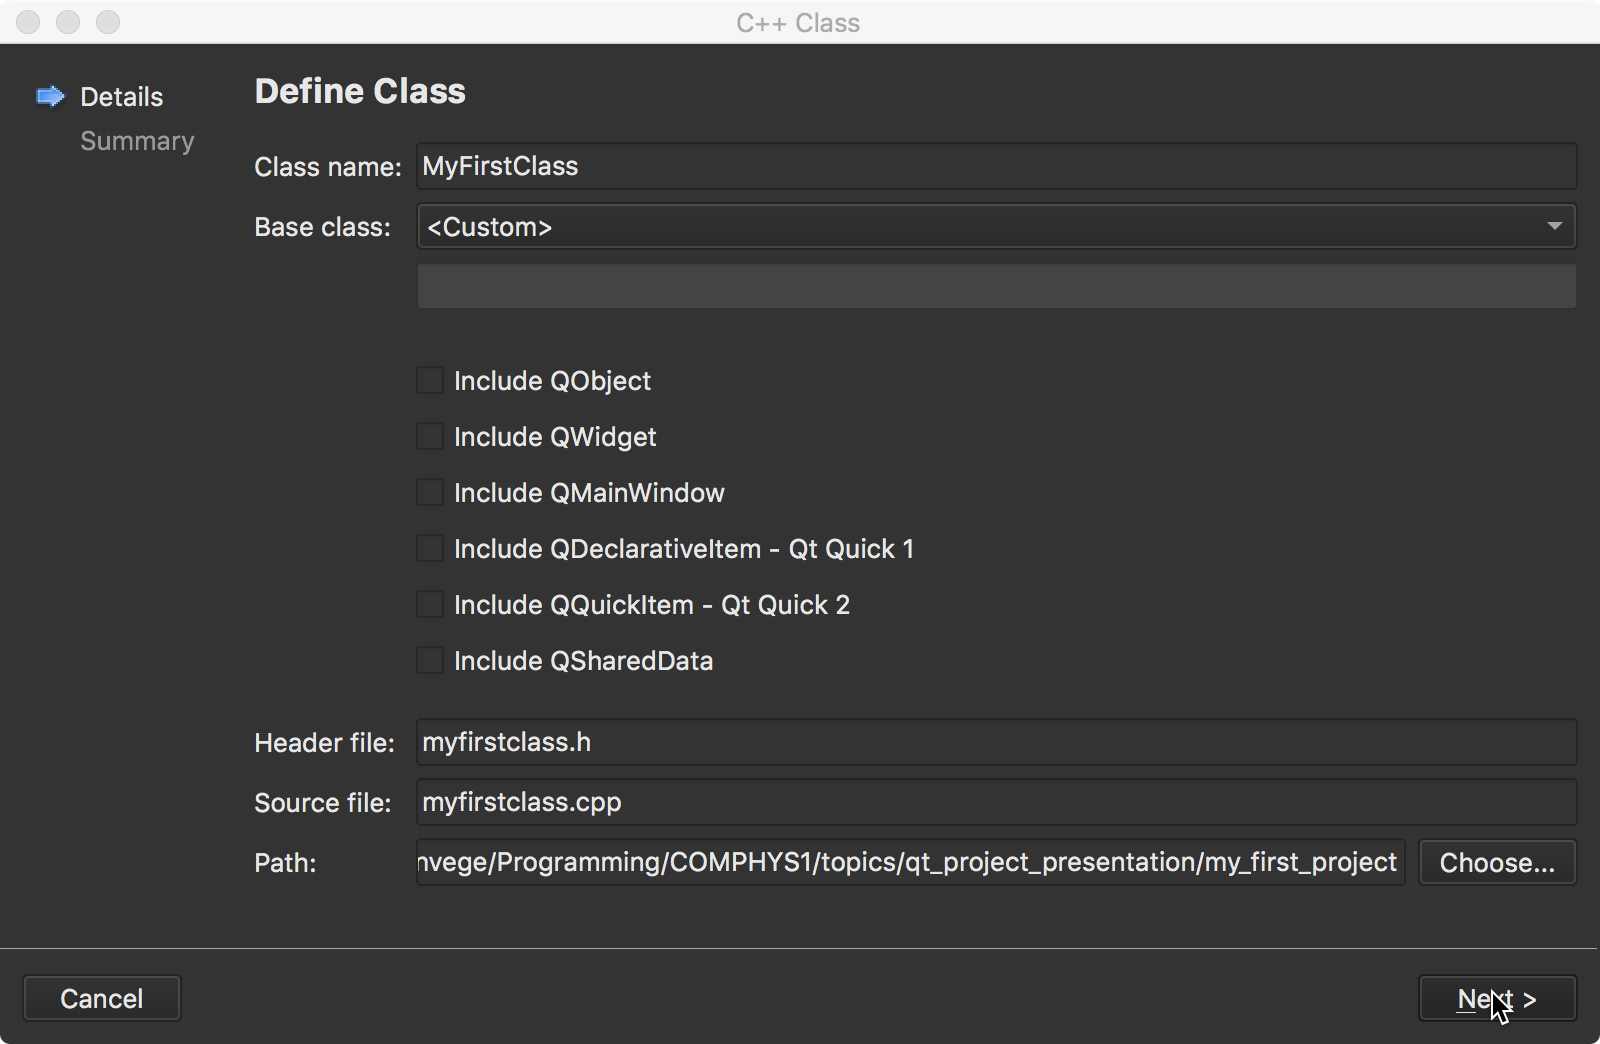
\includegraphics[width=\textwidth]{figures/new_files/first_class.png}
\end{figure}
The files you are including will then be added to the \texttt{.pro} file automatically, and will now look something like,
\lstinputlisting[style=custom-pro-file]{example_project_files/pro_with_files.pro}

\subsection{Adding existing files}
Say we now want to add a files \texttt{"lib.h"} and its functions \texttt{"lib.cpp"} to our project. After taking note of their location, you simply add
\begin{lstlisting}
    <path_to_lib.h>/lib.h
\end{lstlisting}
under \texttt{HEADERS}, and 
\begin{lstlisting}
    <path_to_lib.cpp>/lib.cpp
\end{lstlisting}
under \texttt{SOURCES} in the \texttt{.pro} file. Then you include the file by writing \texttt{\#include "lib.h"} in the file you need it in. \footnote{Go \href{https://stackoverflow.com/questions/21593/what-is-the-difference-between-include-filename-and-include-filename}{here} for an explanation for why we use \texttt{"lib.h"} and not \texttt{<lib.h>}.}

\section{Guides to external libraries for Qt}
After introducing the \texttt{.pro} file, we can look at how libraries is including. In the \texttt{.pro} this is done with primarily two commands:
\begin{lstlisting}
    LIBS += -L/<path_to_library> -l<library_name>
    INLCUDEPATH += <path_to_search_for_headers_in>
\end{lstlisting}

\subsection{Armadillo}
\subsubsection{Installation}
\begin{itemize}
    \item \textbf{Windows}. Look at \href{https://d1b10bmlvqabco.cloudfront.net/attach/j6owewp05ym46p/i8xgc5x4yhoyo/j7ayyo45oocq/blas_lapack_solution_windows.pdf}{this guide} for how to install Armadillo on Windows.
    \item \textbf{Mac}. Install Armadillo by simply typing,
    \begin{lstlisting}
        $ brew install armadillo
    \end{lstlisting}
    in the terminal.
    \item \textbf{Ubuntu}. To install Armadillo on Ubuntu, use
    \begin{lstlisting}
        $ sudo apt-get install libarmadillo-dev
    \end{lstlisting}
\end{itemize}
\subsubsection{Including Armadillo in Qt Creator}
\begin{itemize}
    \item \textbf{Mac}. To include Armadillo on Mac in Qt Creator, you have to add following to your \texttt{.pro} file. This is assuming Brew linked Armadillo correctly and installed all dependencies.
    \begin{lstlisting}
        INCLUDEPATH += /usr/local/include
        LIBS += -L/usr/local/lib -llapack -lblas -larmadillo
    \end{lstlisting}
    The path was used here is the path provided by Brew when typing 
    \begin{lstlisting}
        brew info armadillo
    \end{lstlisting}
    After adding the path go to \textit{Build} at the top, and select \textit{Run qmake}.
    \item \textbf{Ubuntu}. After installing the required libraries, simply include
    \begin{lstlisting}
        LIBS += -llapack -lblas -larmadillo
    \end{lstlisting}
    in your \texttt{.pro} file.
    \item \textbf{Windows}. See post on Piazza or go to the bottom of the same document listed in under the installation of Armadillo.
\end{itemize}
To include Armadillo in your \CC program, go to your \texttt{.pro} file and add the following,

An example of a full \texttt{.pro} file on Mac would be
\begin{lstlisting}
TEMPLATE = app
CONFIG += console c++11
CONFIG -= app_bundle
CONFIG -= qt

SOURCES += \
    main.cpp

INCLUDEPATH += /usr/local/include
LIBS += -L/usr/local/lib 
LIBS += -llapack -lblas -larmadillo
\end{lstlisting}

\subsubsection{Troubleshooting}
\begin{itemize}
    \item \textbf{Mac}. If you run into an issue where you get \texttt{Image not found} at run time, try to reinstall \texttt{arpack} and Armadillo with brew. 
\end{itemize}

\subsection{OpenMP}
OpenMP is a method of parallelizing code.

\subsection{MPI}

\section{Profiling your code}
Two profiling methods will be presented in this section,
\begin{itemize}
    \item \textit{Memory profiling}. Will check if any memory is lost. I.e. you forget to de-allocate any memory.
    \item \textit{Function profiling}. Will check the time spent in each function.
\end{itemize}

Methods for profiling code can be found at Qt Wiki for \href{https://wiki.qt.io/Profiling_and_Memory_Checking_Tools}{Profiling and Memory Checking Tools}. Here, we will present Valgrind as the choice of profiler.

To view output of the Valgrind profiler(in case you do not use Qt Creator), use KCacheGrind(or QCacheGrind for Mac users) which can be found \href{https://github.com/KDE/kcachegrind}{here}.

\subsection{Installing Valgrind}
\subsubsection{Mac}
Install Valgrind with brew,
\begin{lstlisting}
$ brew install valgrind
\end{lstlisting}
If you use MacOS High Sierra(> 10.13), you might get an error on the form of,
\begin{lstlisting}
valgrind: mmap-FIXED(0x7fff5f400000, 8388608) failed in UME (load_unixthread1) with error 22 (Invalid argument).
\end{lstlisting}
The fix is to uninstall Valgrind and reinstall with the \texttt{--HEAD}.
\begin{lstlisting}
$ brew uninstall valgrind
$ brew install valgrind --HEAD
\end{lstlisting}

\subsubsection{Ubuntu}
Simple use
\begin{lstlisting}
$ sudo apt-get install valgrind
\end{lstlisting}
and you should have it.

\subsection{Installing K/QCachegrind}
\subsubsection{Mac}
\begin{lstlisting}
$ brew install kcachegrind
\end{lstlisting}

\subsubsection{Ubuntu}
\begin{lstlisting}
$ sudo apt-get install kcachegrind
\end{lstlisting}

\subsection{Running Valgrind memory check(memcheck)}
\subsubsection{Qt Creator}
In Qt Creator, first compile your program in debug mode. Then select Analyze -> Valgrind Memory Analyzer with GDB. If the drop-down panel is something else than Debugger click it and select memcheck. If it does not start, click Run.

The output will then on the shape of
\begin{figure}[H]
    \centering
    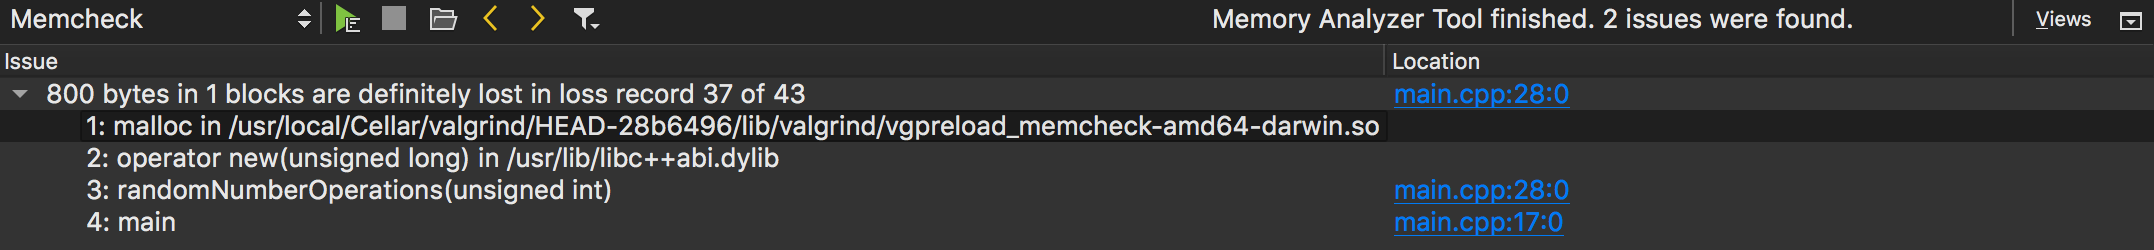
\includegraphics[width=\textwidth]{figures/valgrind-qt/valgrind}
\end{figure}

\subsubsection{Terminal}
If you want to run in terminal, you might want to have your program compiled in debug mode(not required though), and type following 
\begin{lstlisting}
$ valgrind --leak-check=full ./my_executable
\end{lstlisting}
The argument \verb|--leak-check=full| prompts Valgrind to output a detailed overview of the locations of where it detected memory leaks.

Mac users: Valgrind may display many leaks which are related to the OS, and thus can be discarded.

\subsection{Profiling with Valgrind(Callgrind)}
\subsubsection{Qt Creator}
If Qt Creator, you select Analyze $\rightarrow$ Valgrind Function Profiler. Qt Creator should now be profiling your code for you. You result should look something like this:
\begin{figure}[H]
    \centering
    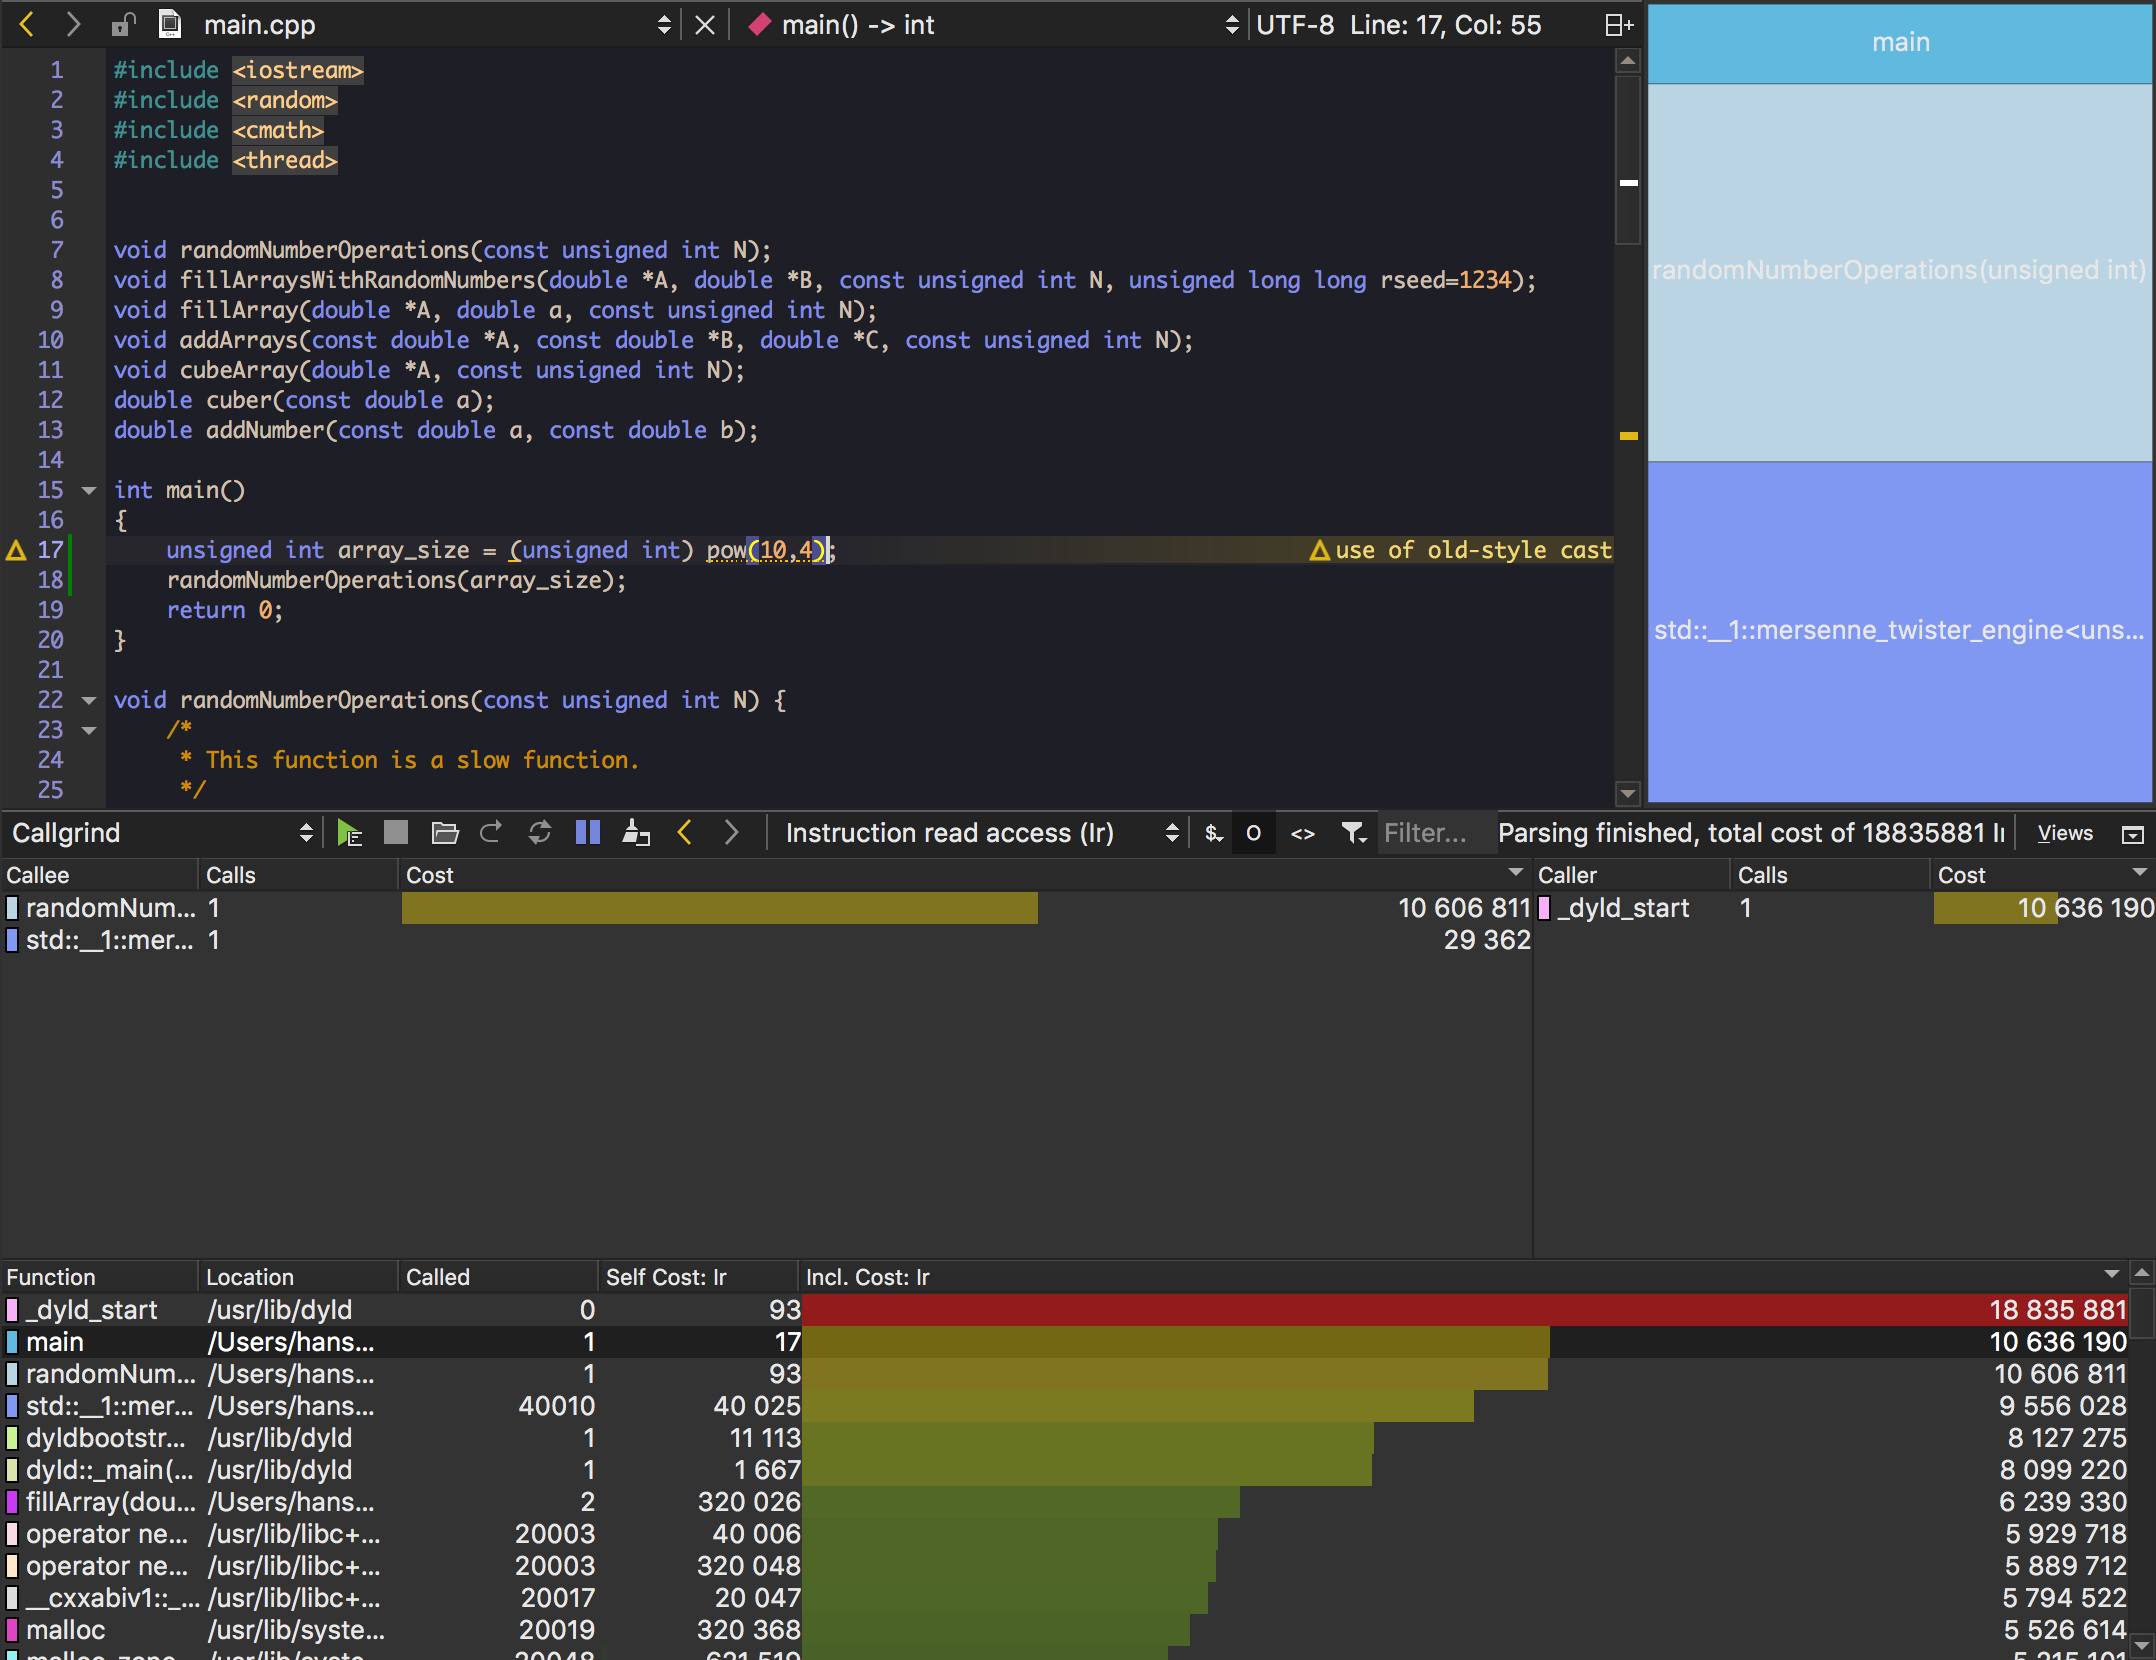
\includegraphics[width=\textwidth]{figures/valgrind-qt/callgrind}
\end{figure}

\subsubsection{Terminal}
To run a Callgrind in terminal, use
\begin{lstlisting}
$ valgrind --tool=callgrind ./my_executable
\end{lstlisting}

This produces an output on the format of \texttt{callgrind.out.<pid>}. The last numbers is just the Process identifier. To view this file (depending on OS), use,
\textit{Mac}:
\begin{lstlisting}
$ qcachegrind callgrind.out.<pid>
\end{lstlisting}
\textit{Ubuntu}:
\begin{lstlisting}
$ kcachegrind callgrind.out.<pid>
\end{lstlisting}


\section{Optimizing your code}
By including \texttt{-march-native} you allow for processor specific compilation.

\texttt{-O3} you will allow get vectorization enabled, together with the optimizations from \texttt{-O2}, \texttt{-O1}, \texttt{-OFast}. 

With \texttt{-fopt-info} you will see what compiler optimizations is performed.


\section{Parallelization}
There are two main roads to parallelize your code: either through \textit{MPI} or through \textit{OpenMP}. 
\subsection{MPI}

\subsubsection{Mac}
To parallelize with MPI, make sure you have OpenMPI installed,
\begin{lstlisting}
$ brew install open-mpi
\end{lstlisting}

\subsubsection{Ubuntu}
To install MPI, simply type,
\begin{lstlisting}
$ sudo apt install mpich
\end{lstlisting}

\subsection{OpenMP}
\subsubsection{Mac}
To parallelize with OpenMP on Mac\footnote{Discussion around how to make OpenMP run on Mac is covered in \href{https://stackoverflow.com/questions/39979836/using-openmp-with-c11-on-mac-os}{this} stackoverflow post}, ensure you have \texttt{libomp}, by using Brew.
\begin{lstlisting}
$ brew install lstlisting
\end{lstlisting}
Then, to compile in terminal, write
\begin{lstlisting}
$ g++ -Xpreprocessor -fopenmp -o <your-program>.o <your-program>.cpp -lomp
\end{lstlisting}
\subsubsection{Ubuntu}
To install OpenMP on Ubuntu, simply type
\begin{lstlisting}
$ apt-get install libomp-dev
\end{lstlisting}


\end{document}